
\lstinputlisting[language=bash,basicstyle=\tiny]{python_codes/fieldstone_69/keywords}

\begin{center}
Code at \url{https://github.com/cedrict/fieldstone/tree/master/python_codes/fieldstone_69}
\end{center}

\par\noindent\rule{\textwidth}{0.4pt}

I have re-implemented most parts of the GHOST code \cite{thie18} in python. 
This stone only generates a spherical shells (so no hollow sphere mesh), 
i.e. all nodes are on the same radius. 

\begin{center}
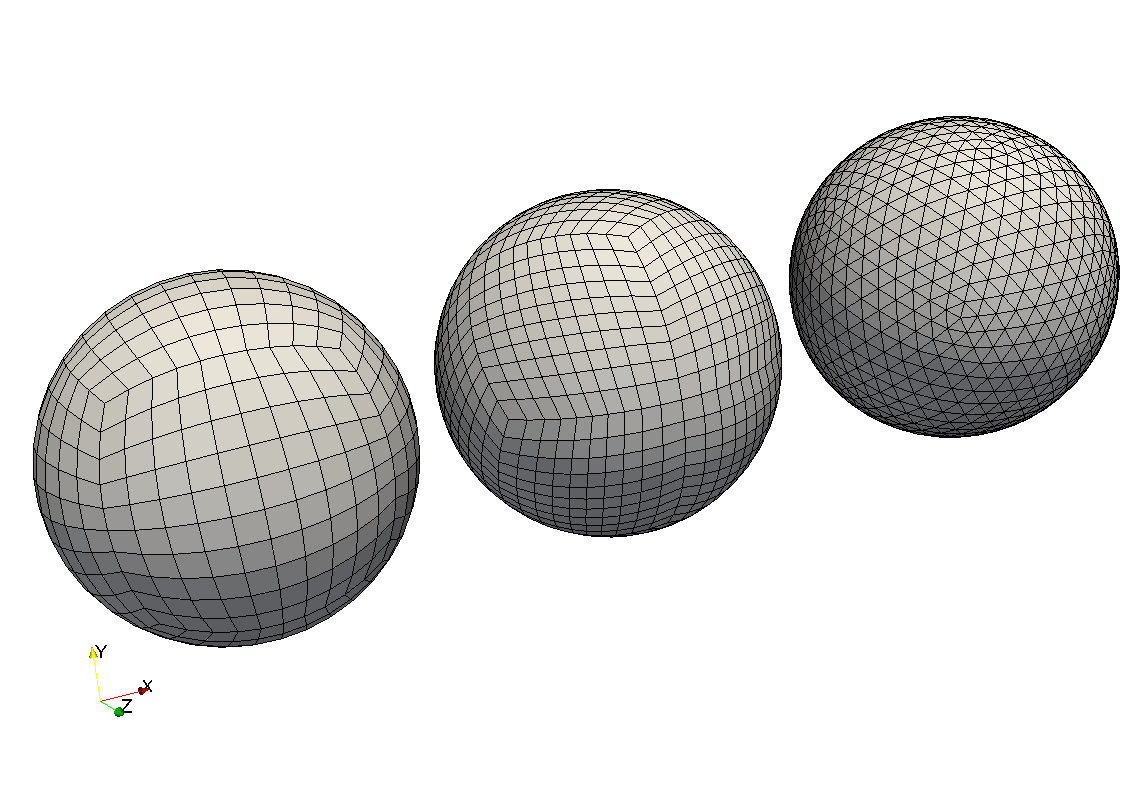
\includegraphics[width=12cm]{python_codes/fieldstone_69/images/shells}\\
{\captionfont Left: cubed sphere; Middle: Citcom mesh; Right: Icosahedral mesh. 
All three at level=10.}
\end{center}

There are three python codes: {\sl rivers.py}, {\sl coastlines.py} and {\sl plate\_boundaries.py} which allow the user to choose 
a radius on which the data will projected. There are 3 folders {\sl rivers}, {\sl coastlines} and {\sl plate\_boundaries} which contain the relevant data per 'continent', i.e. 
Africa, Asia, Europe, North America and South America in this case. 
I have downloaded these data off the internet some 15 years ago and I can unfortunately not assign these references, except 
for the plate boundaries which come from Bird (2003) \cite{bird03}.

\begin{center}
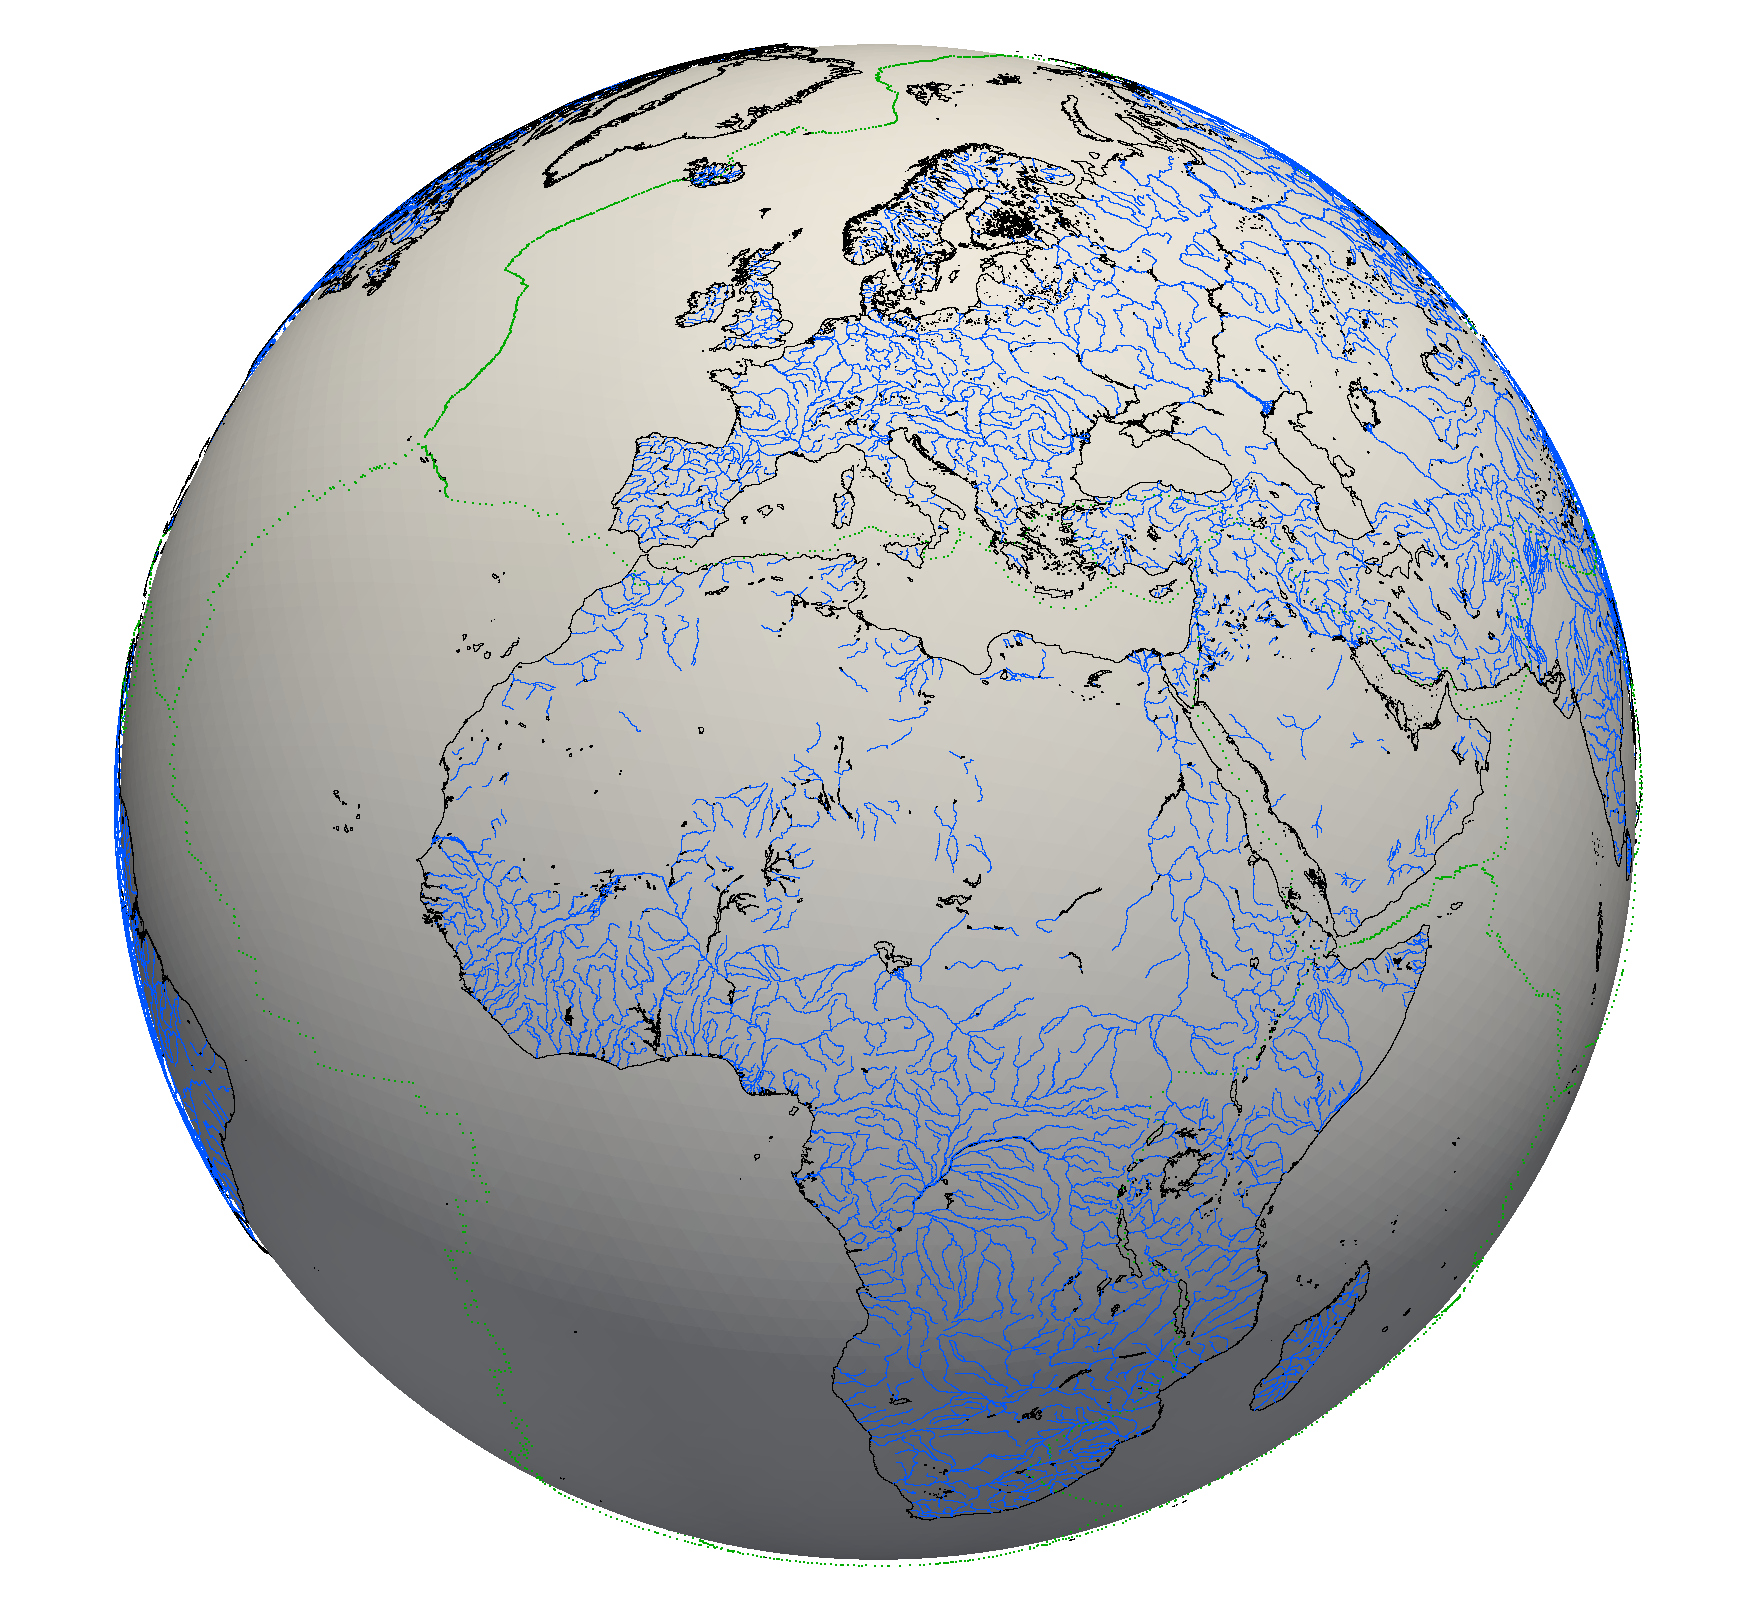
\includegraphics[width=7cm]{python_codes/fieldstone_69/images/01}
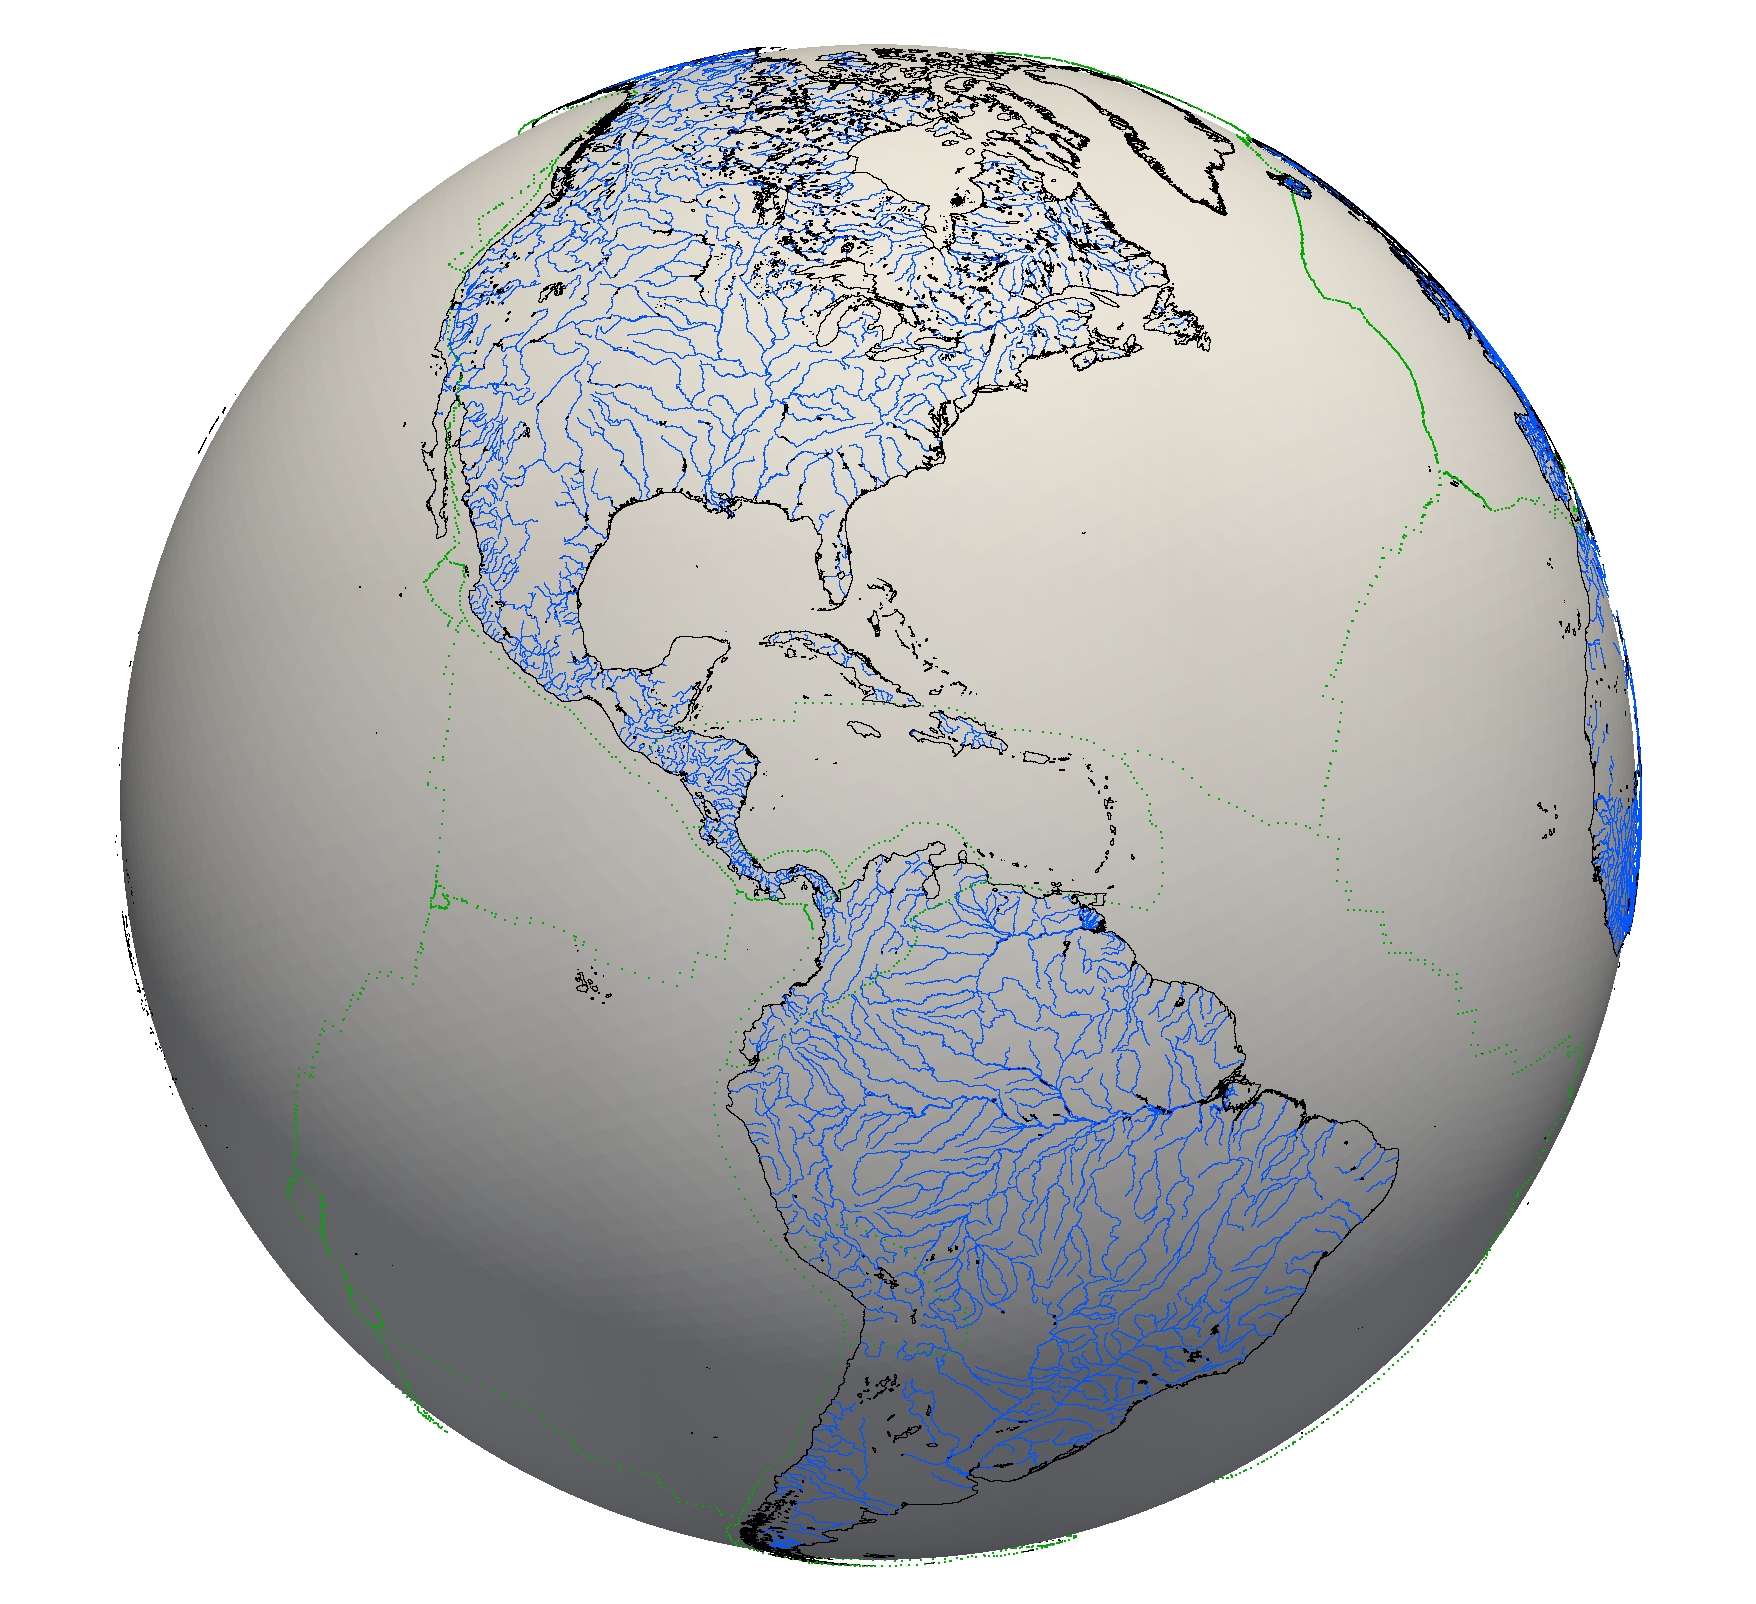
\includegraphics[width=7cm]{python_codes/fieldstone_69/images/02}\\
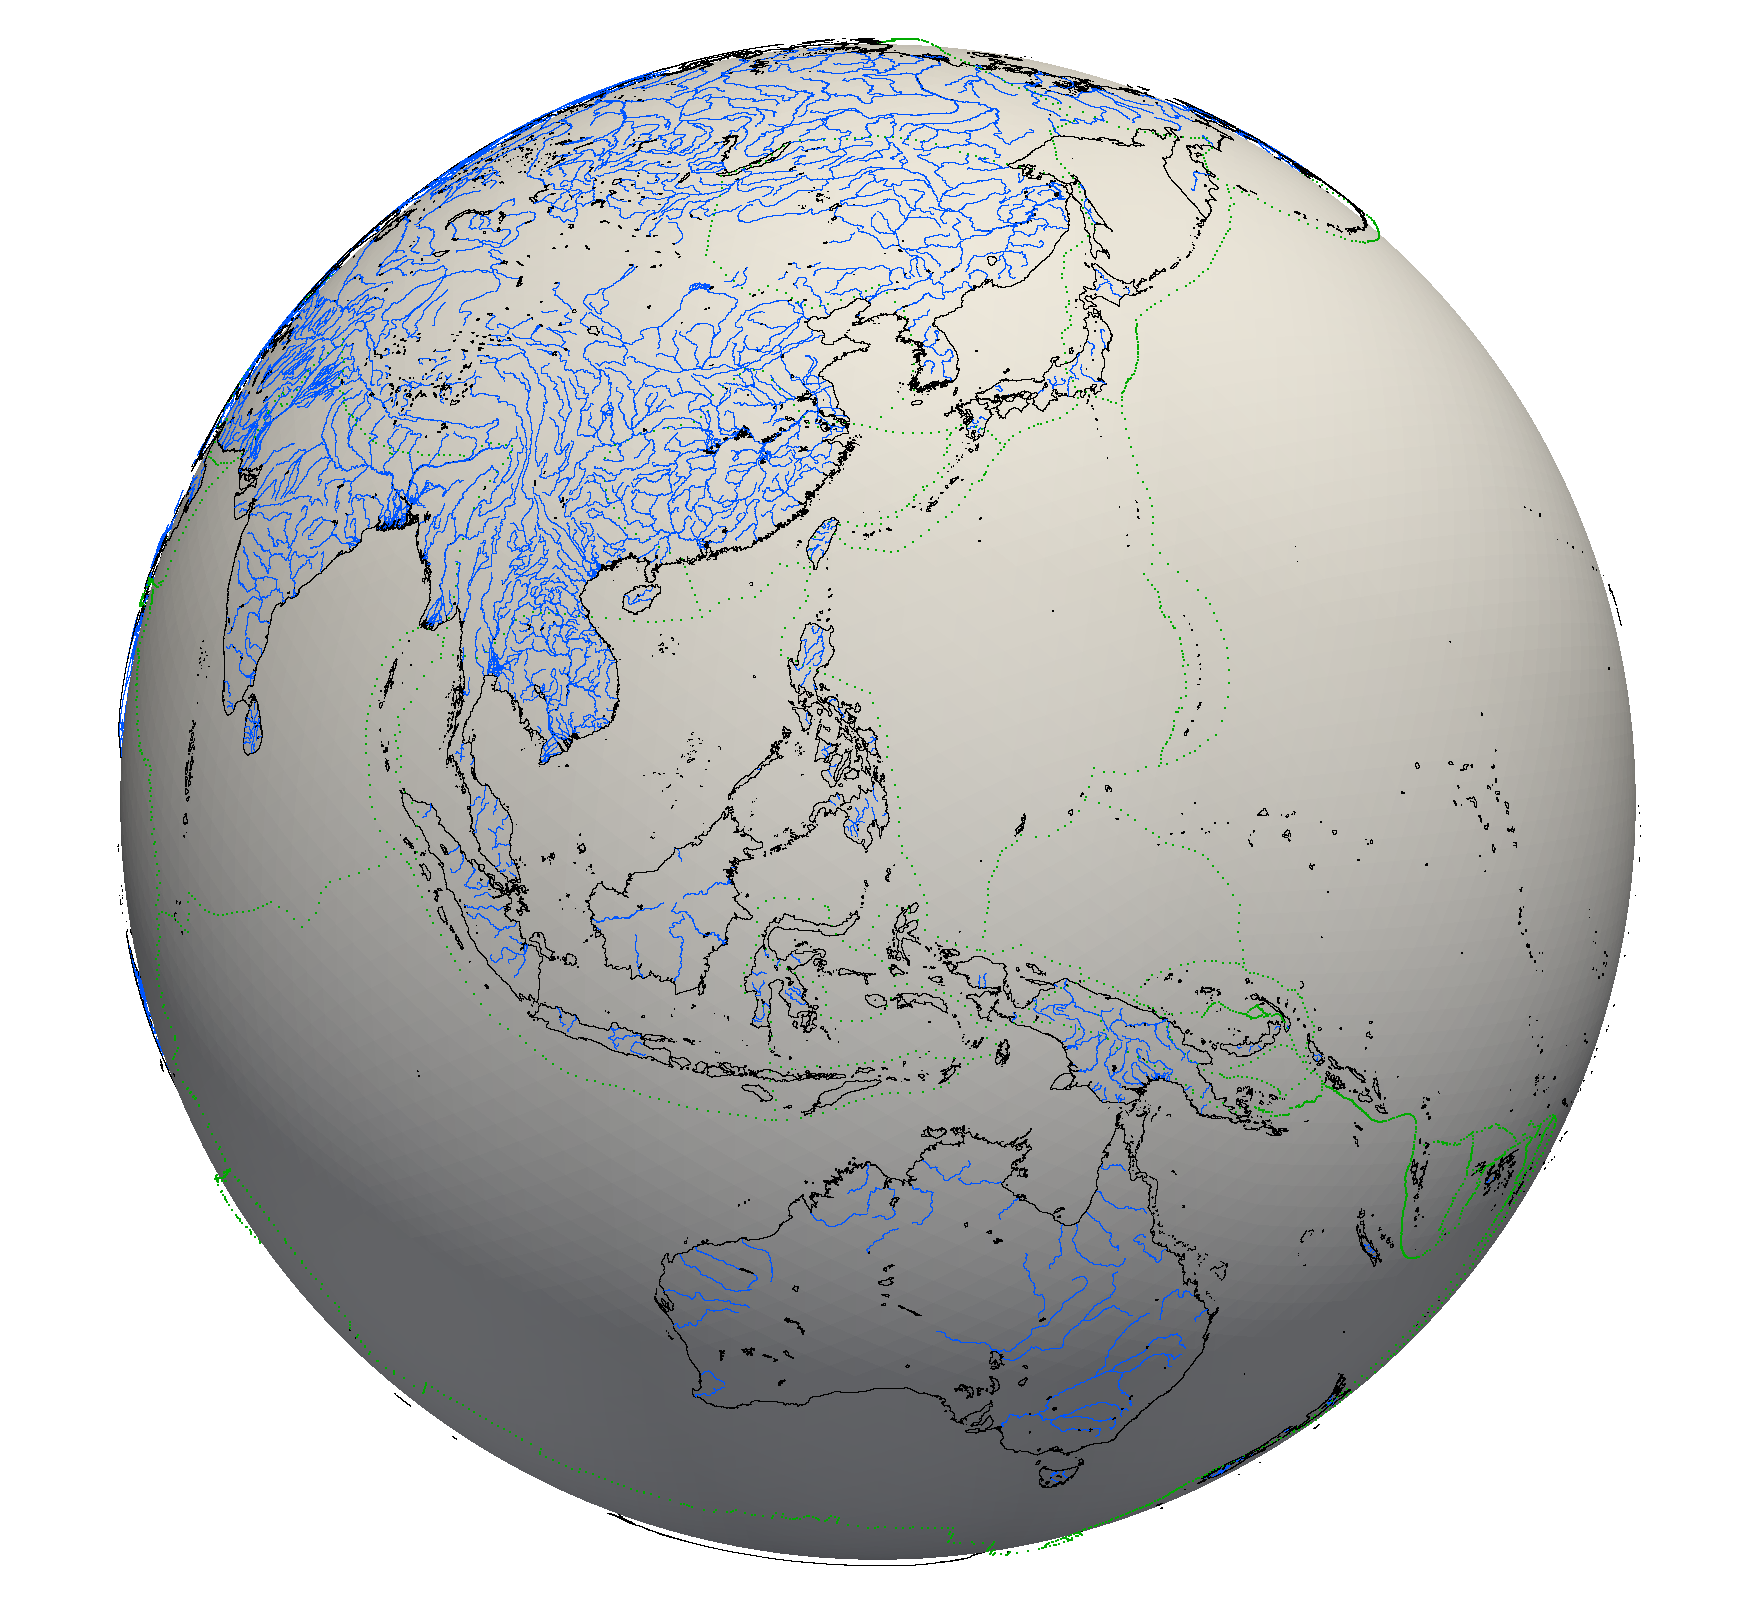
\includegraphics[width=7cm]{python_codes/fieldstone_69/images/03}
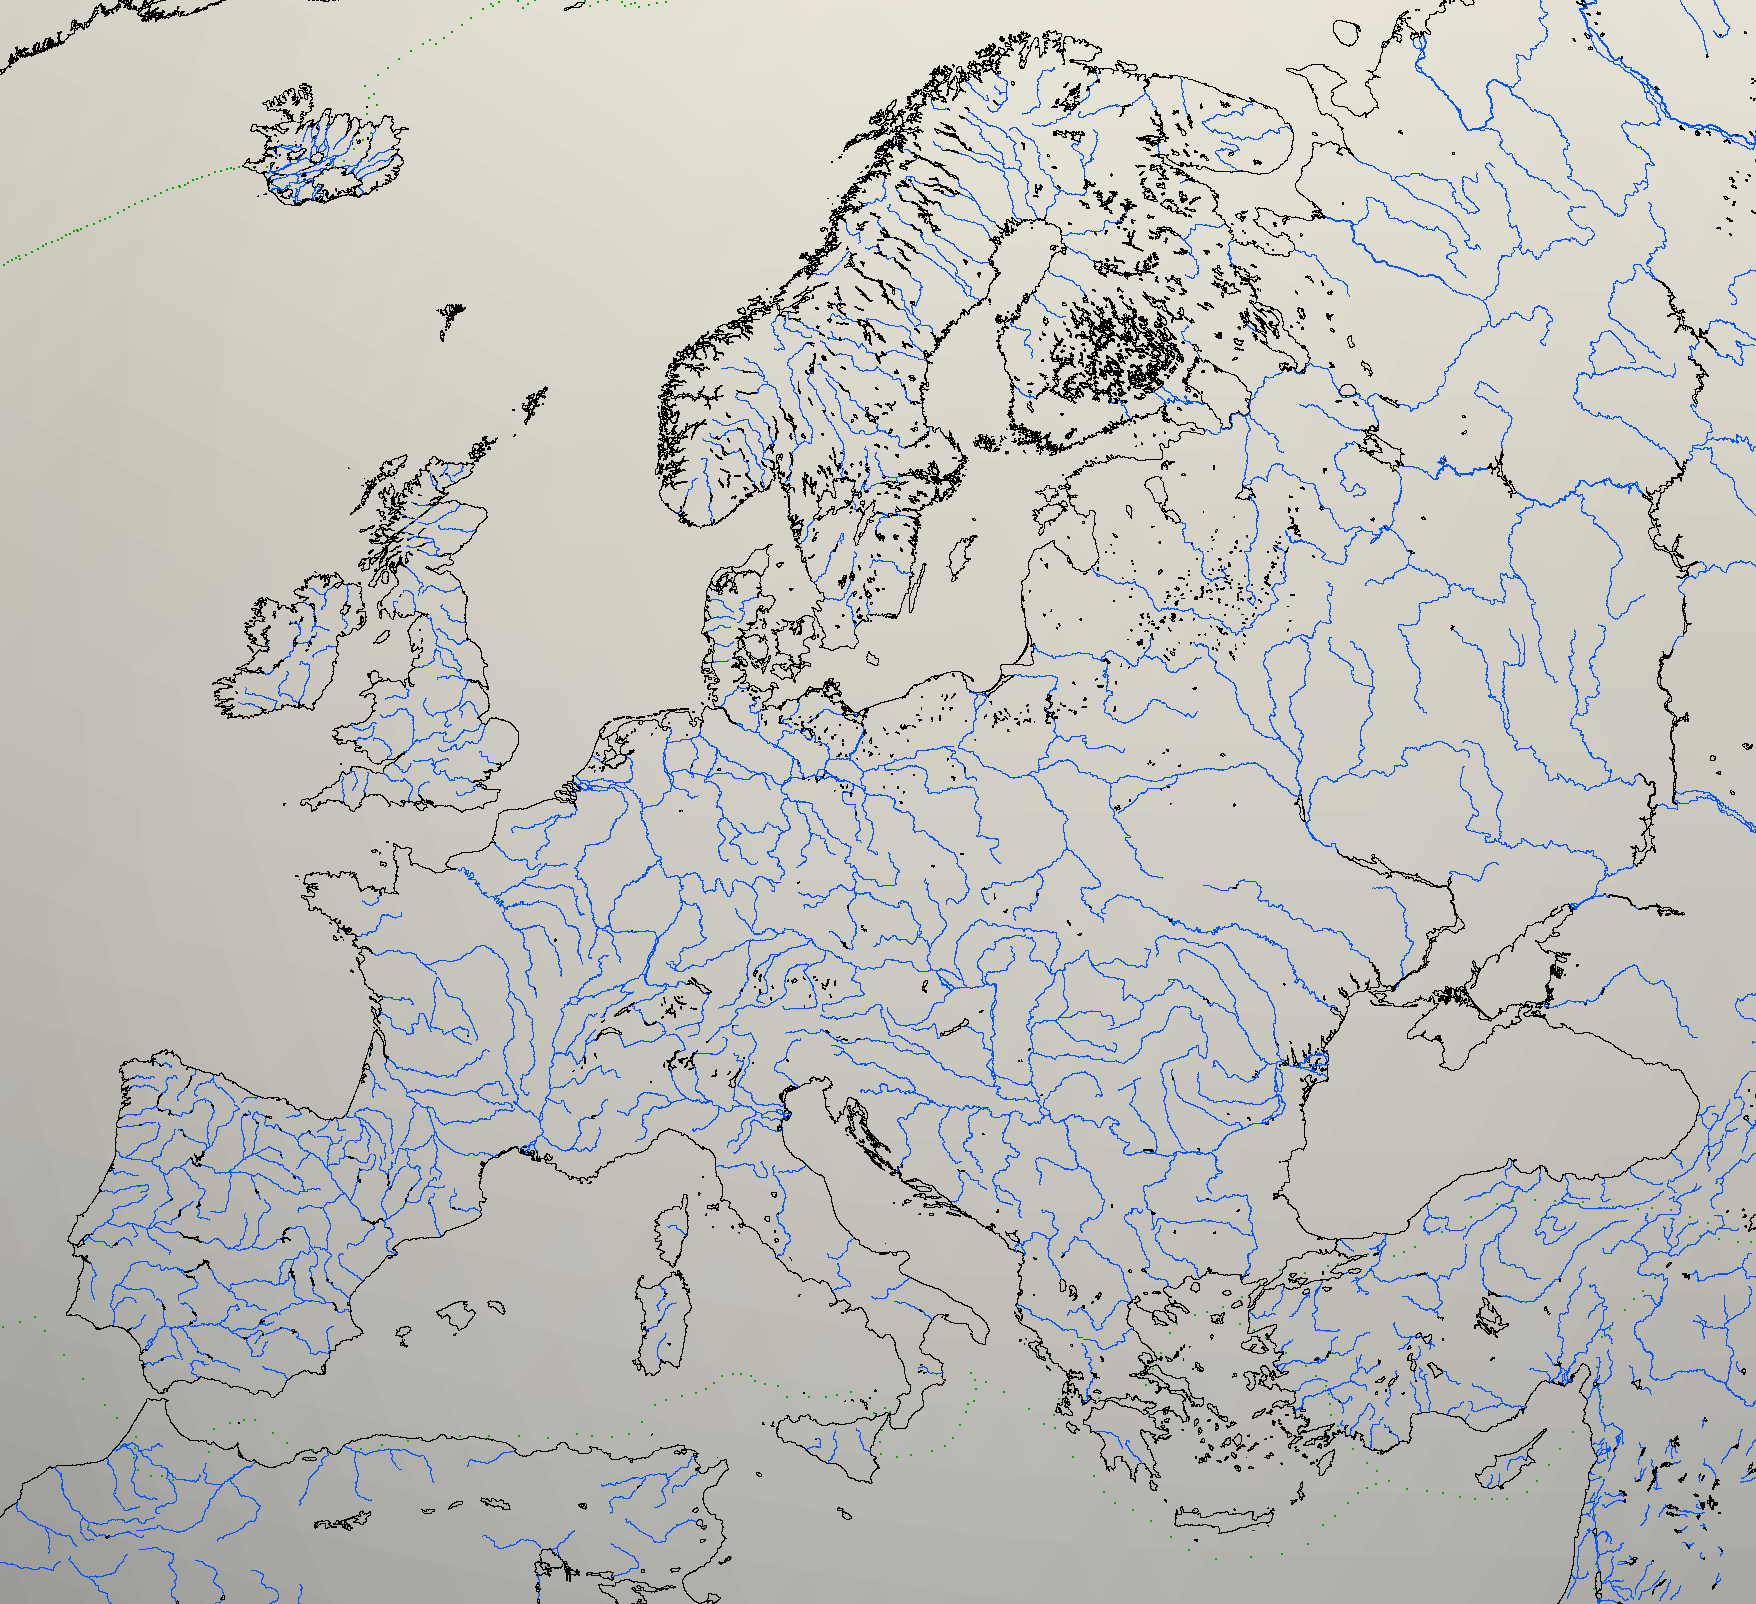
\includegraphics[width=7cm]{python_codes/fieldstone_69/images/04}
\end{center}

The data for the Digital Elevation Model (DEM) 
is available at \url{http://www.temis.nl/data/topo/dem2grid.html}
which has a 0.25 degree resolution (1440x720 points).

\begin{center}
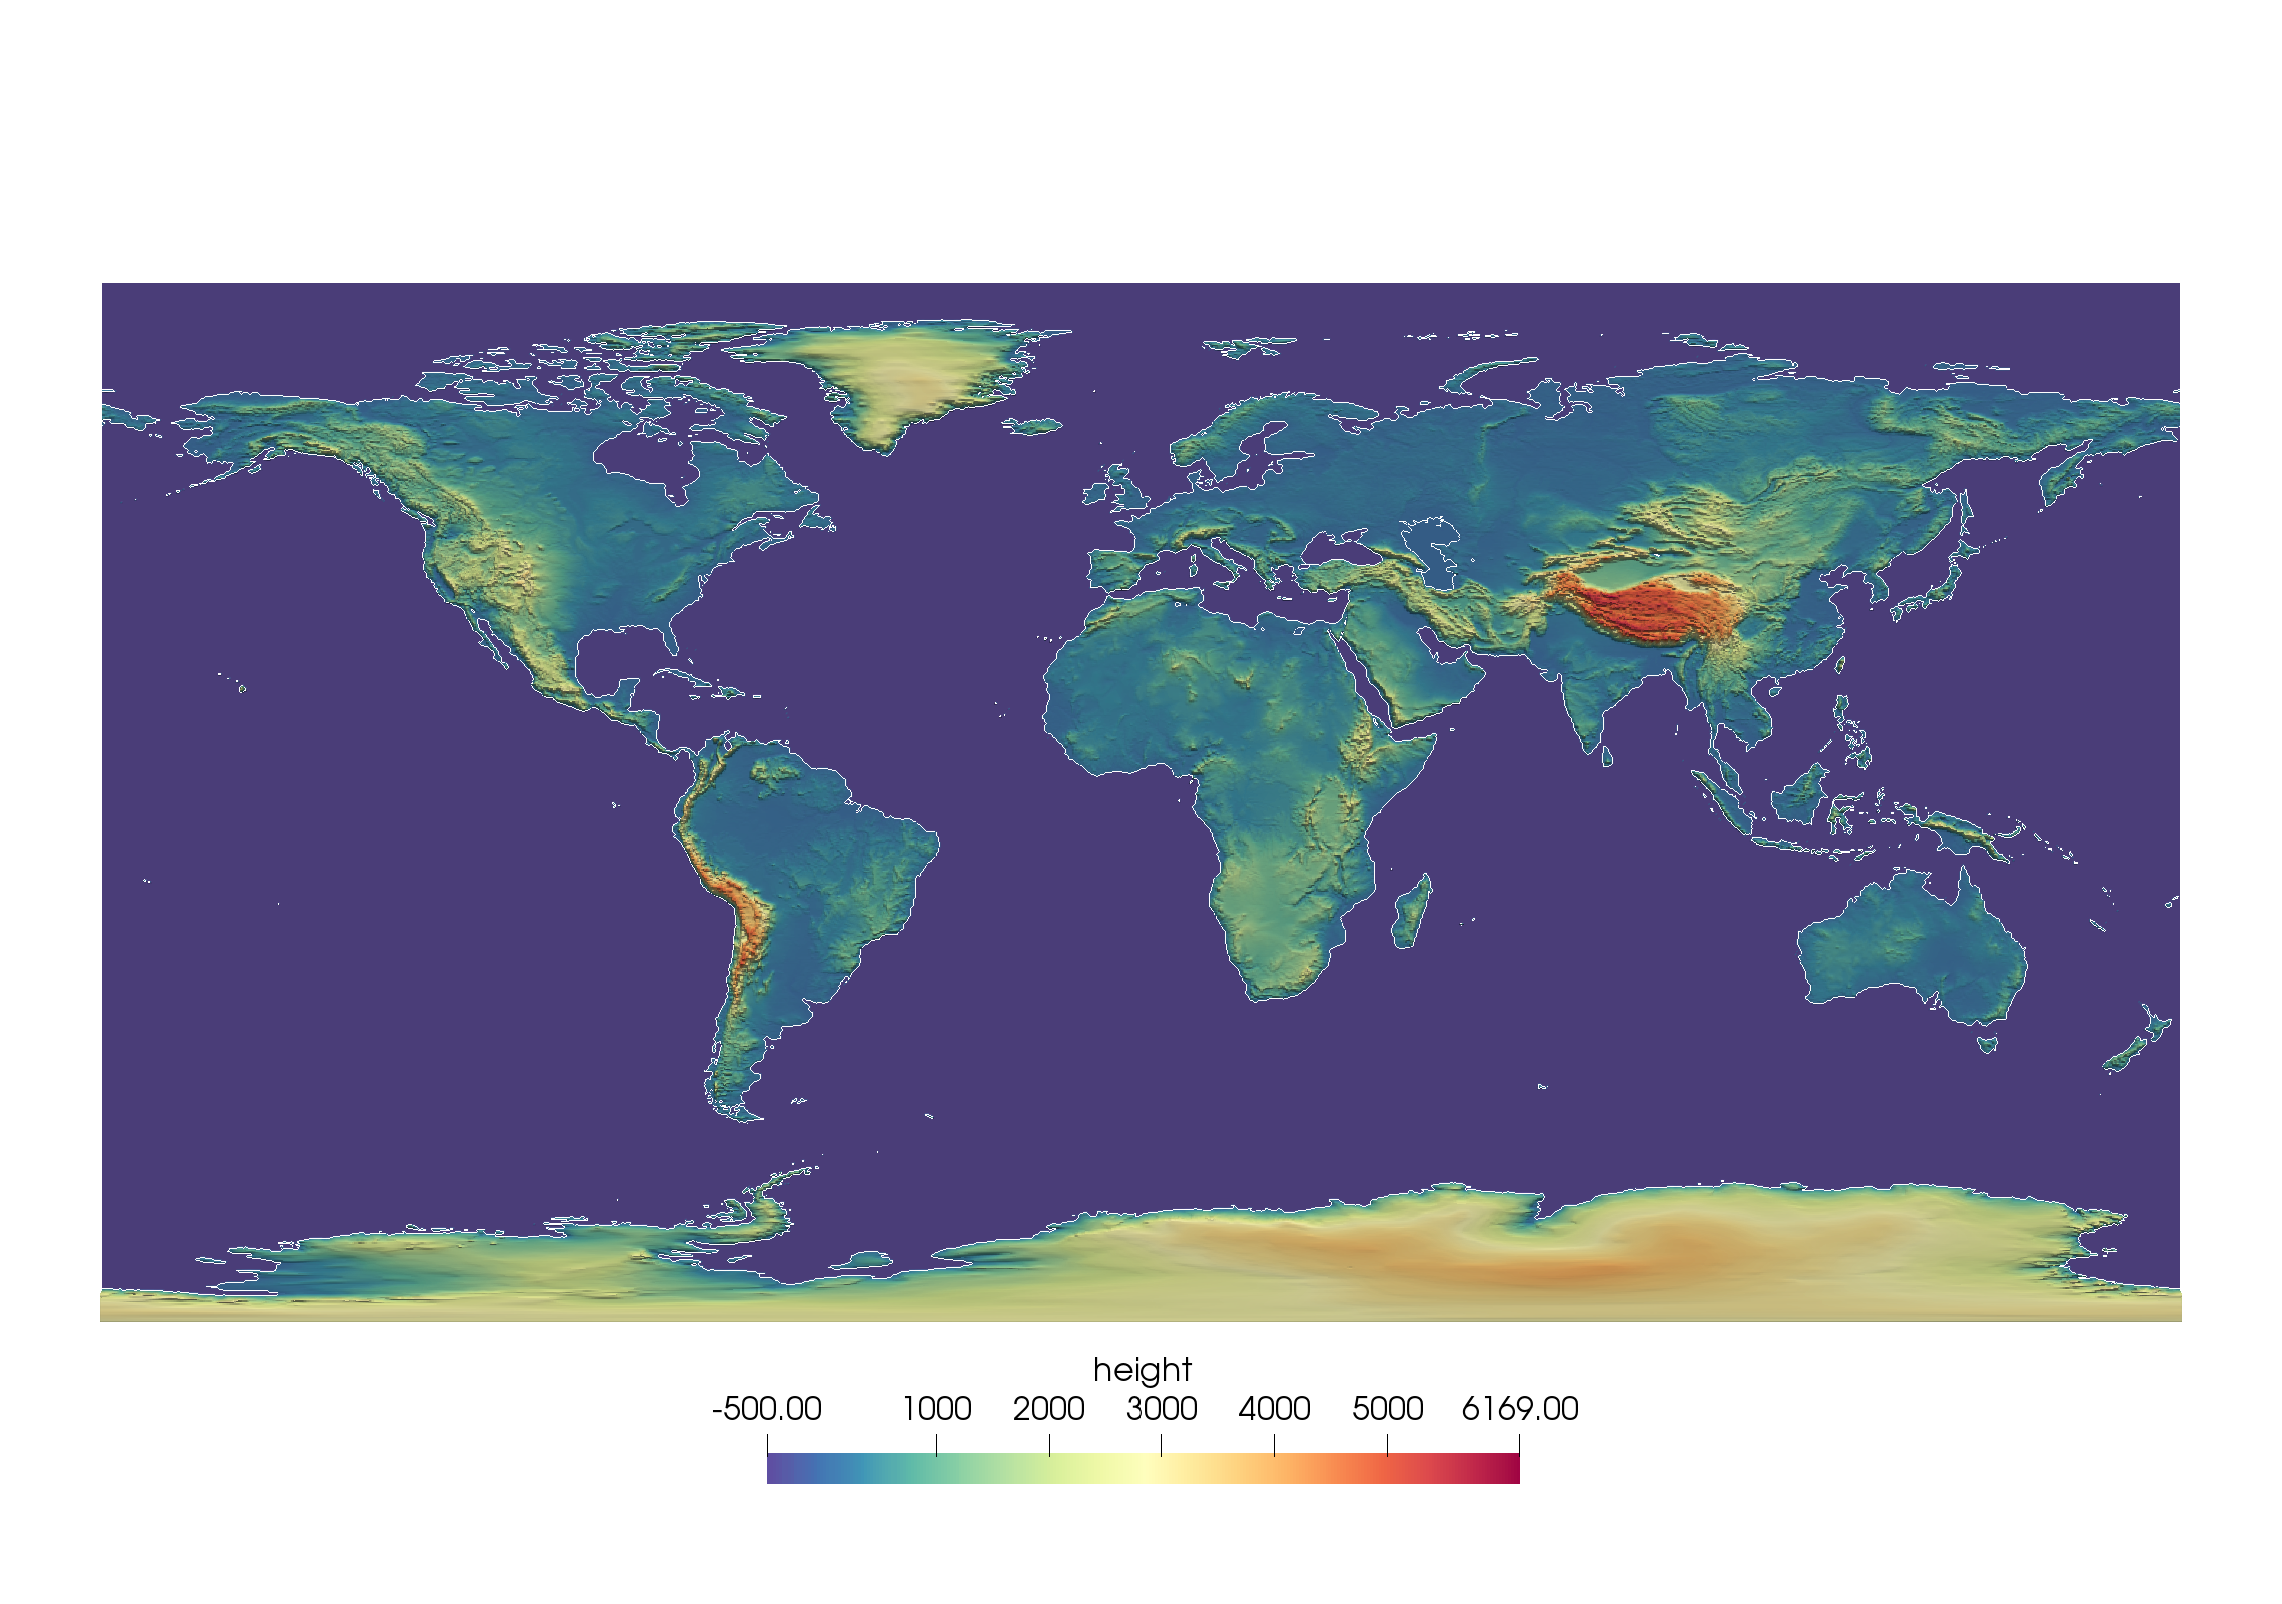
\includegraphics[width=14cm]{python_codes/fieldstone_69/topo/topo.png}\\
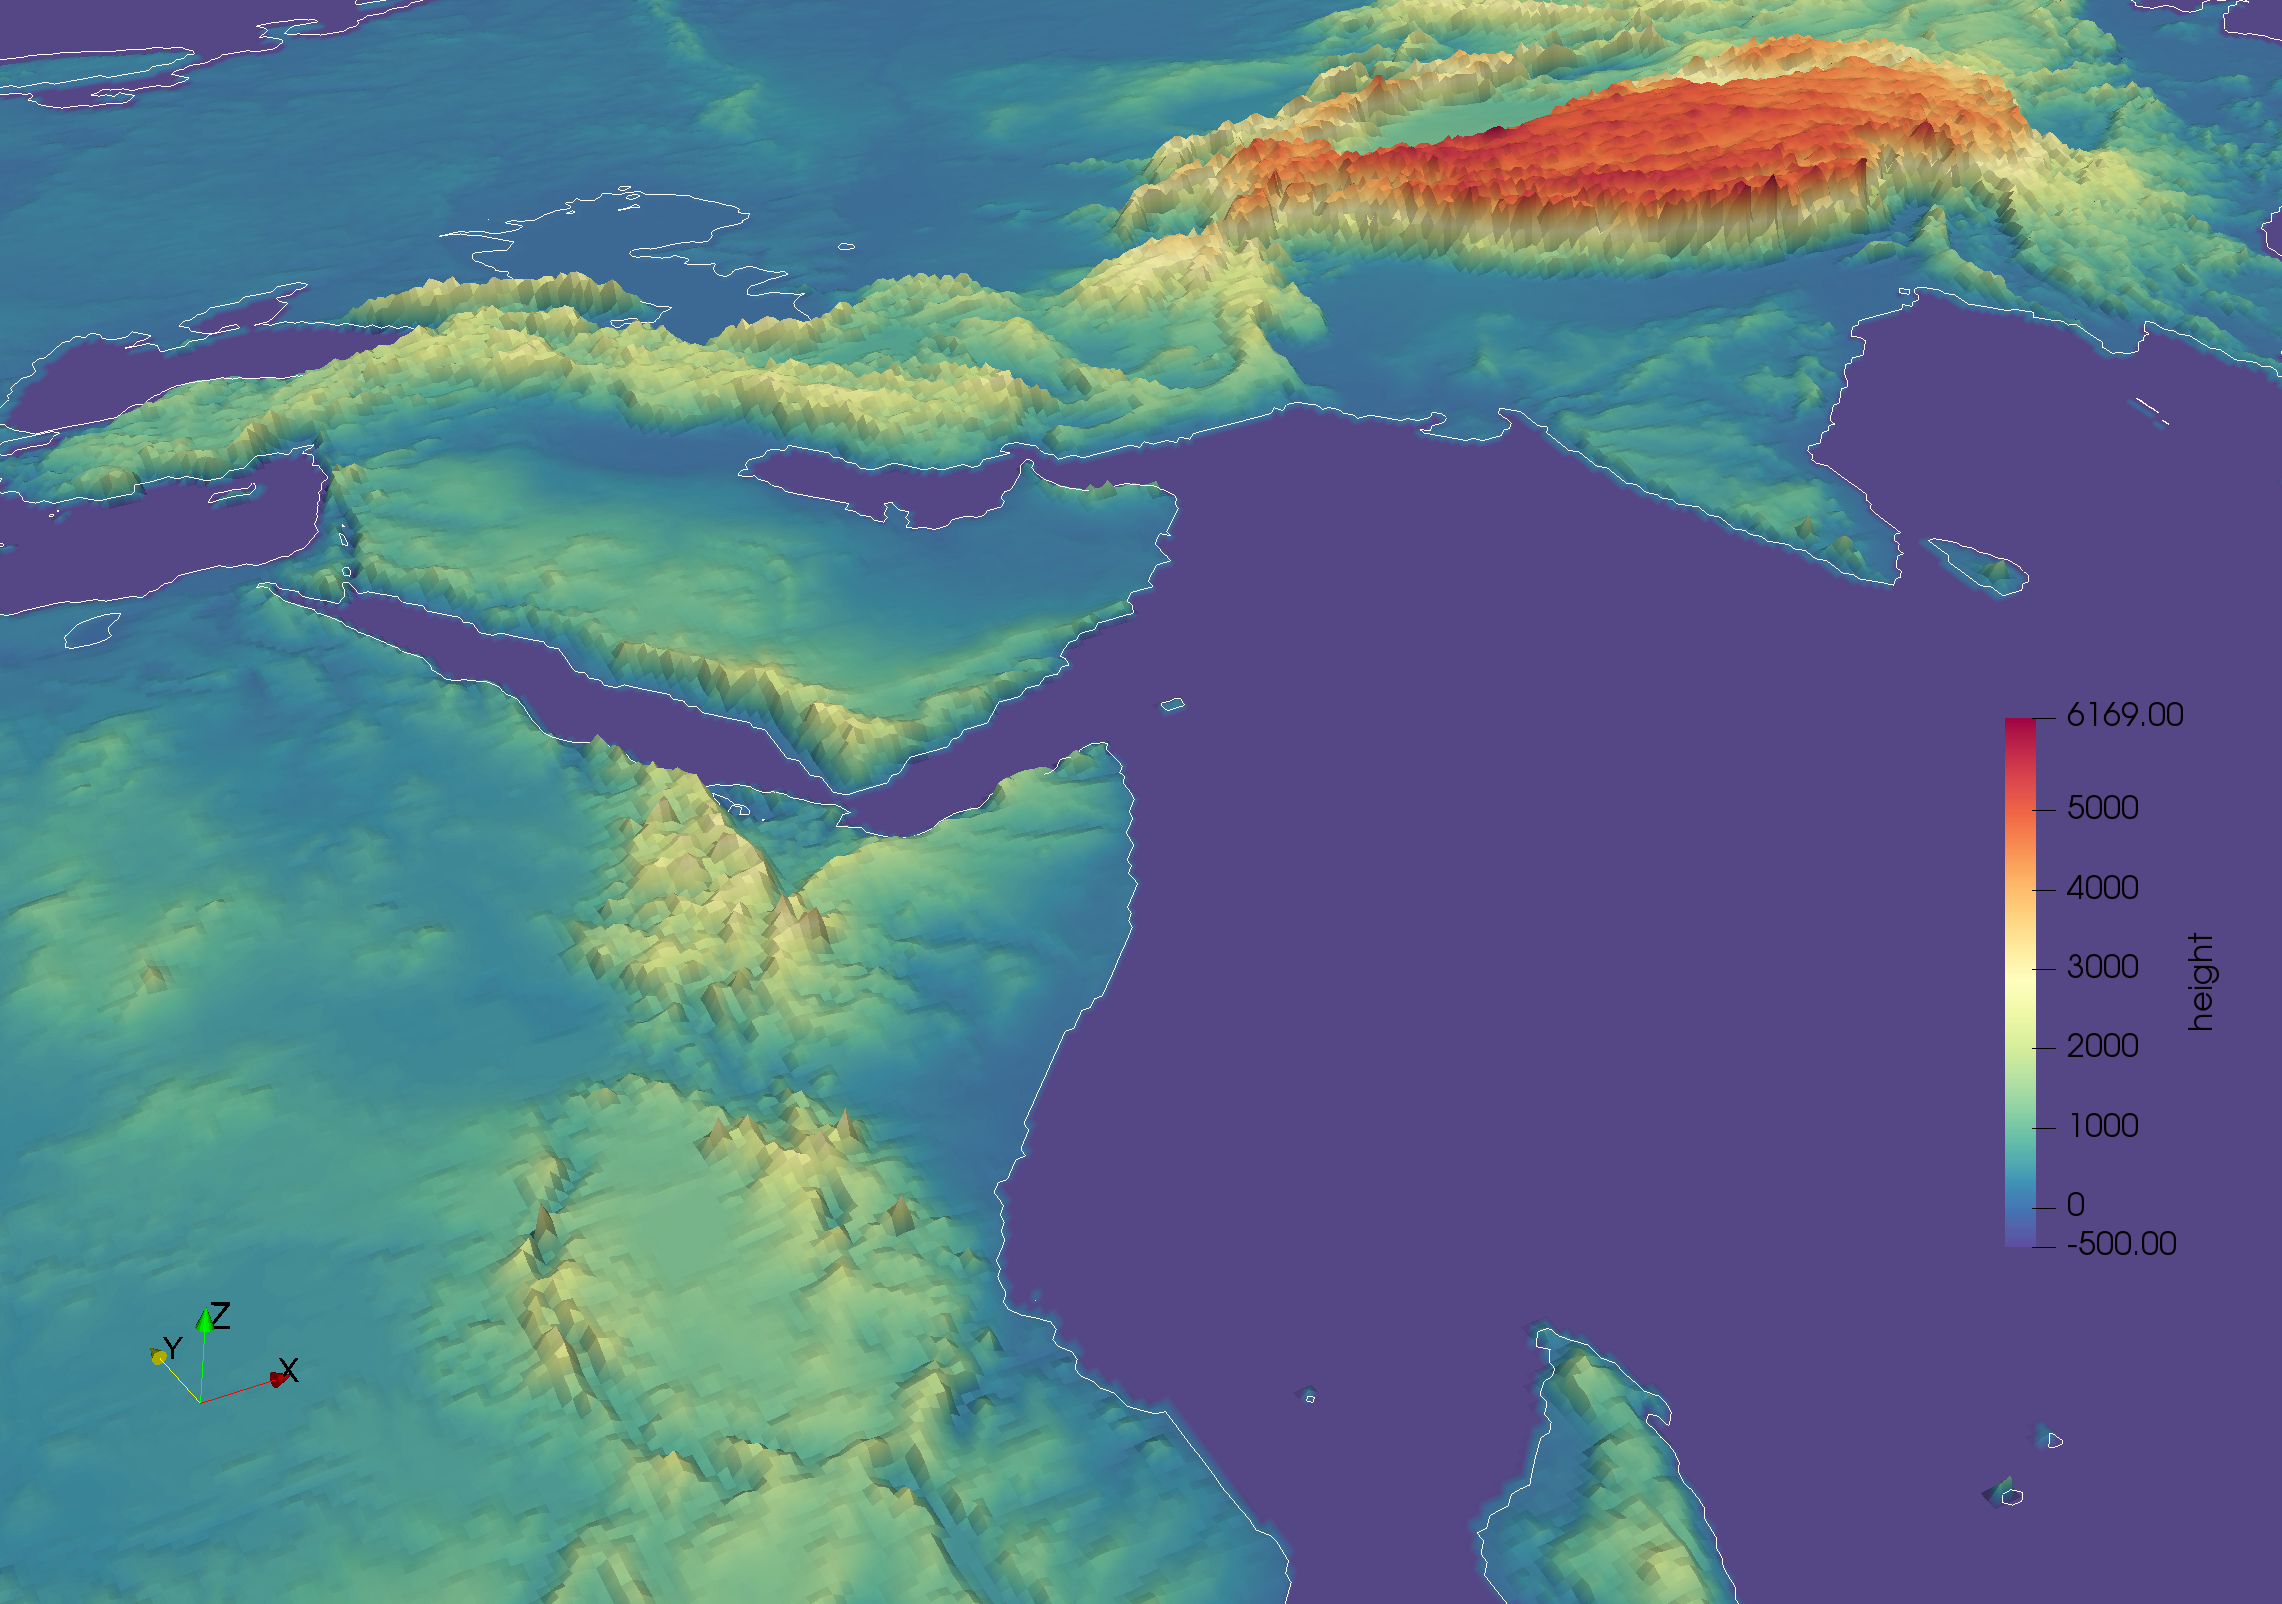
\includegraphics[width=7cm]{python_codes/fieldstone_69/topo/topo2.png}
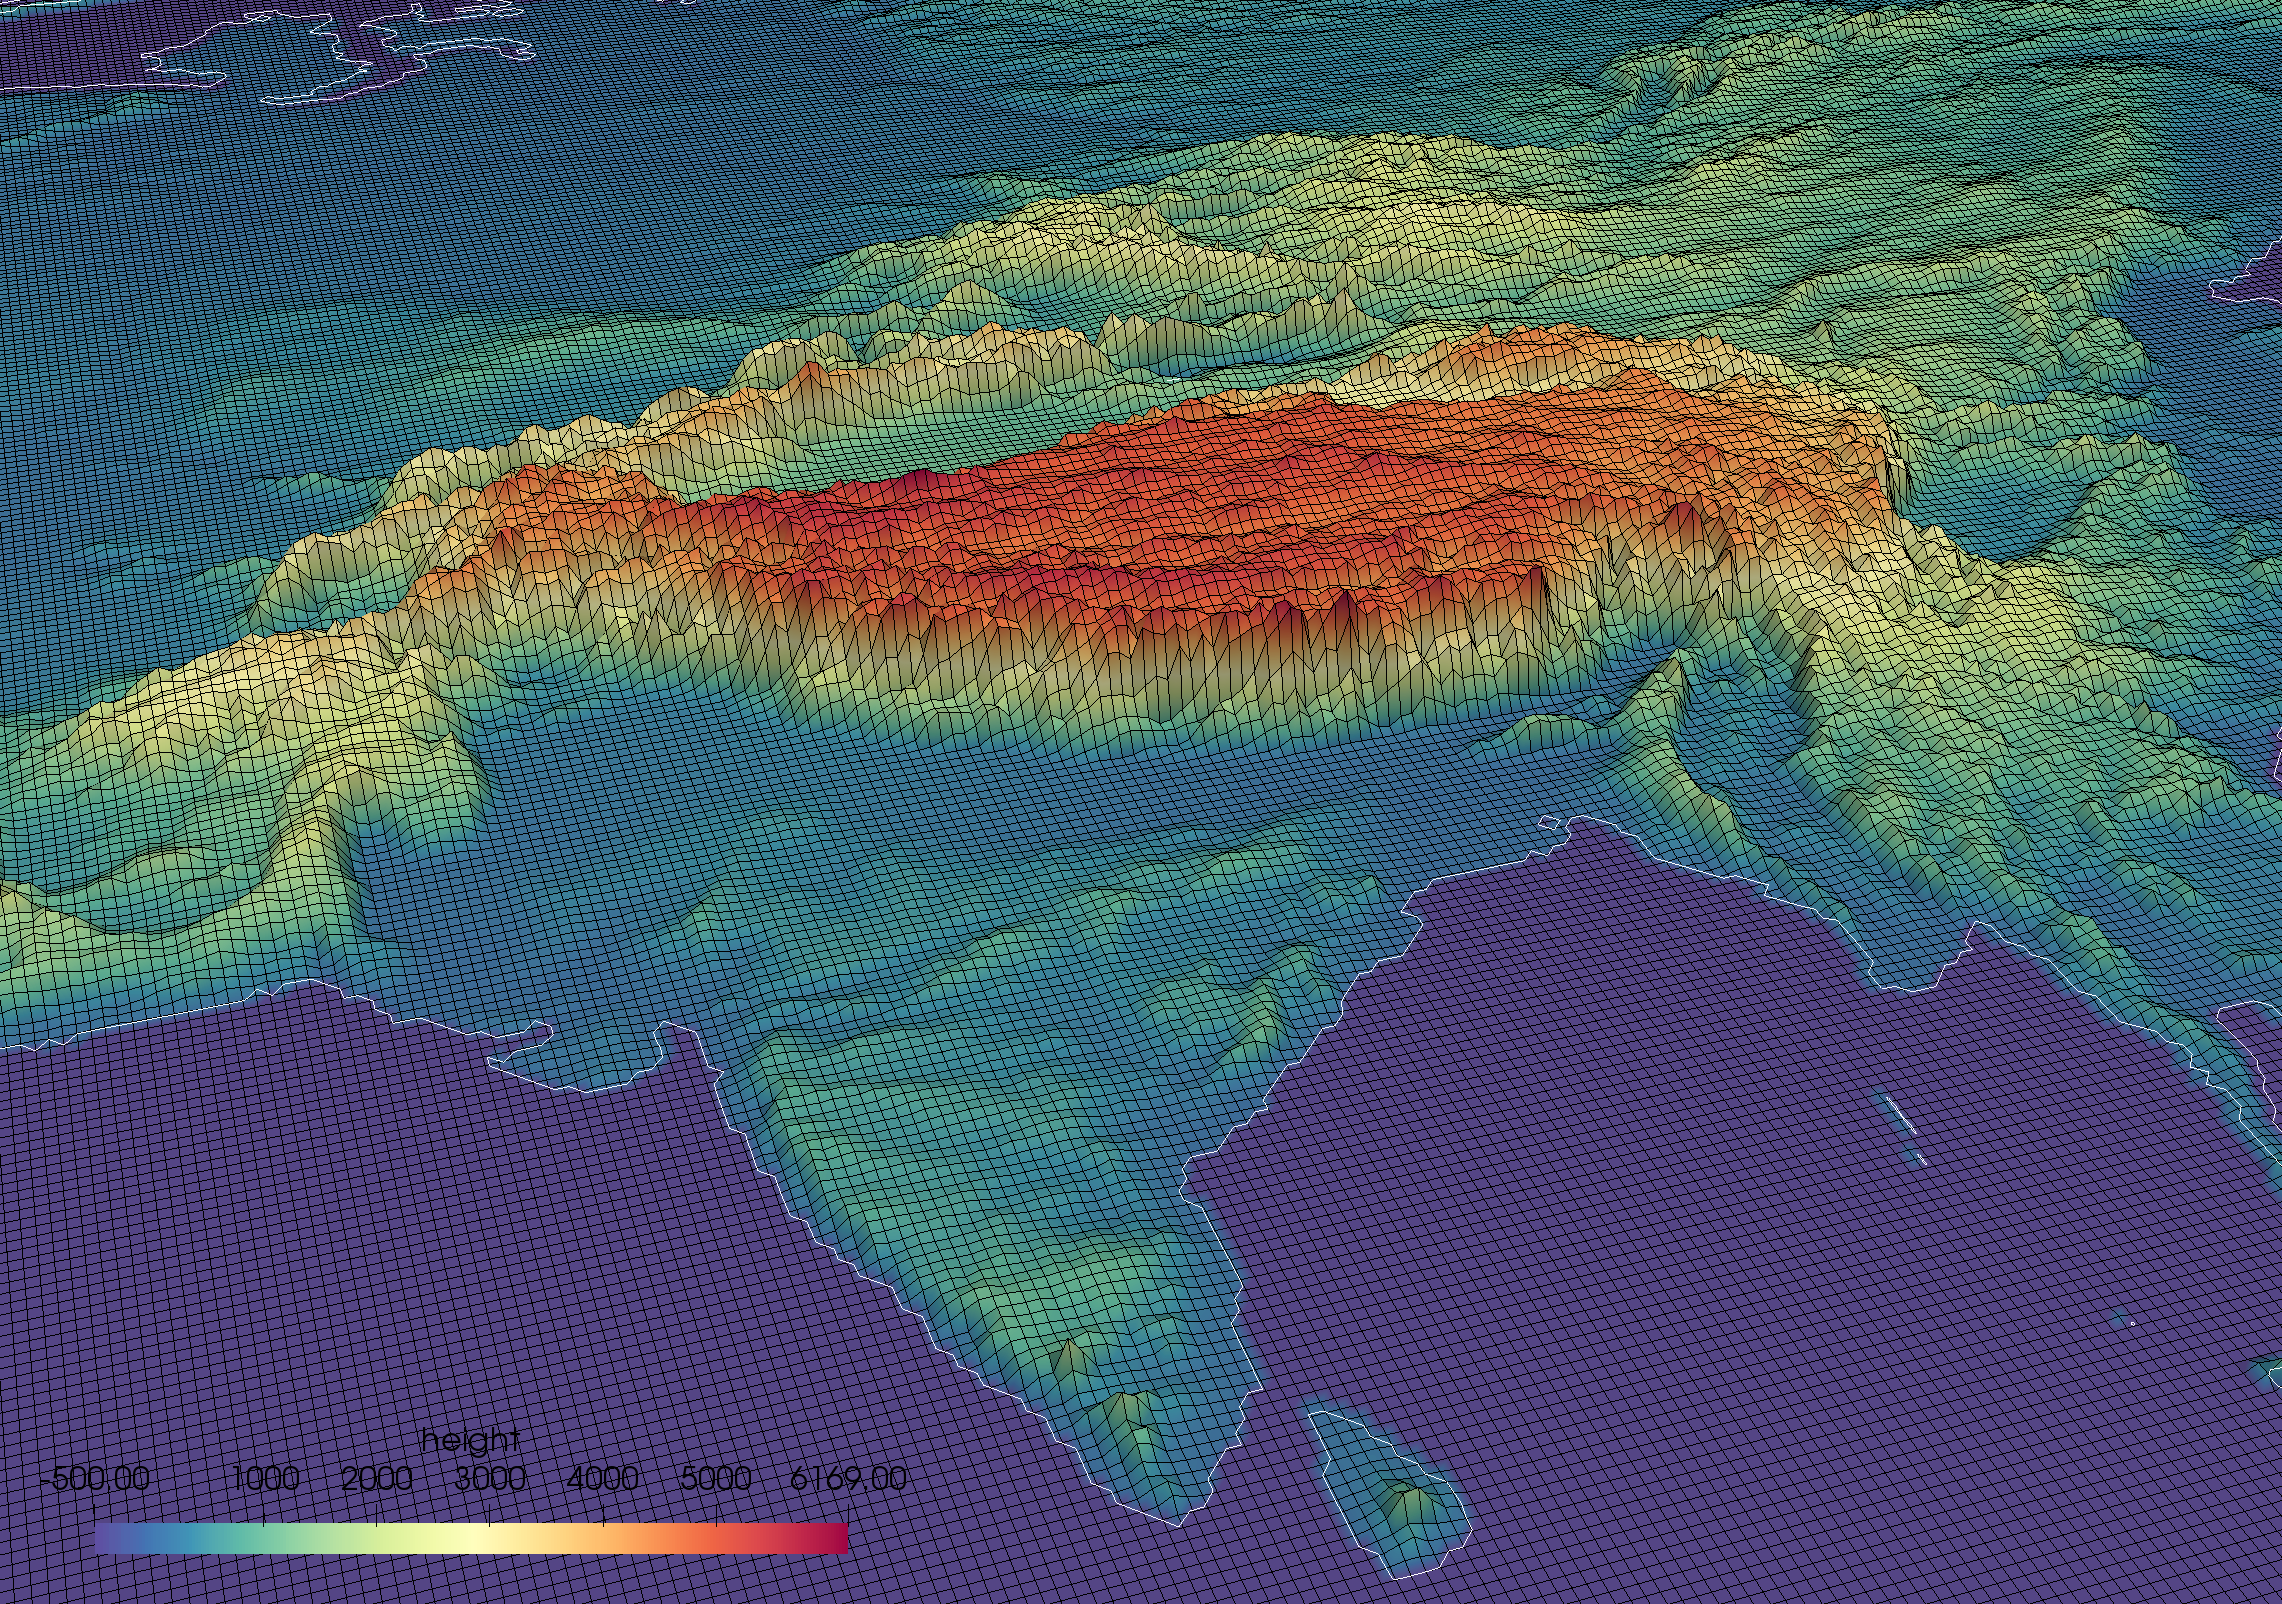
\includegraphics[width=7cm]{python_codes/fieldstone_69/topo/topo3.png}\\
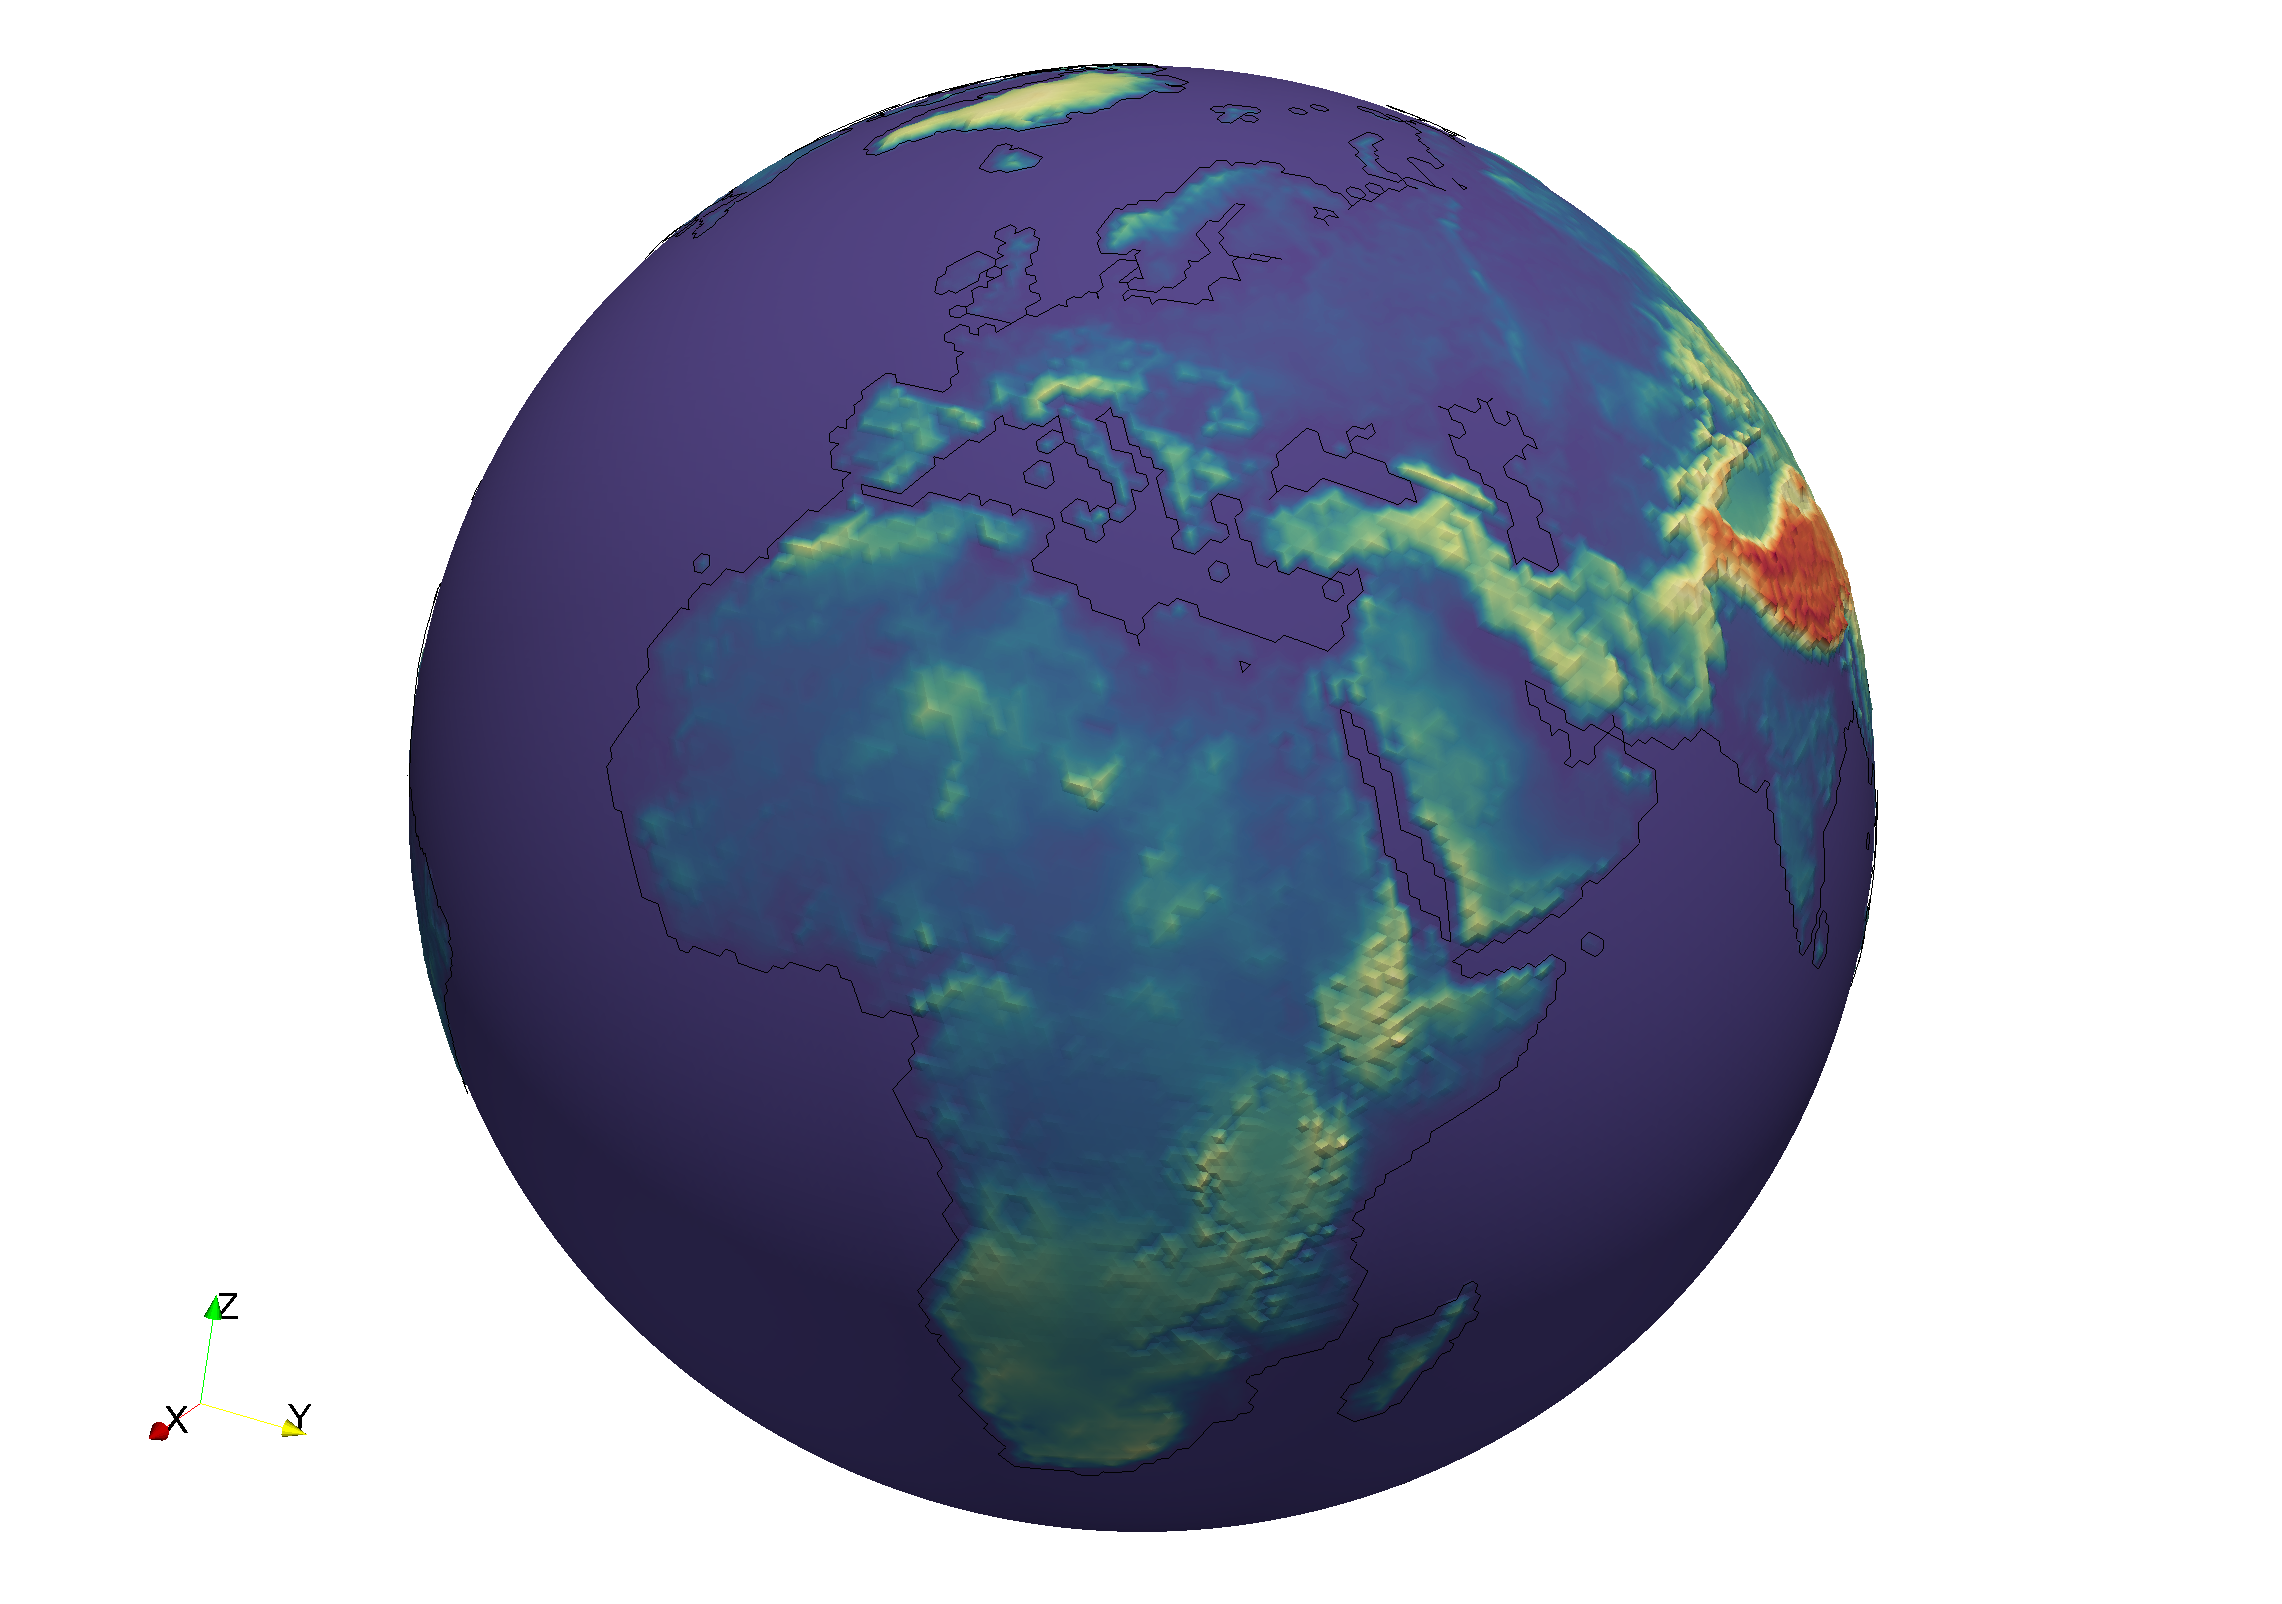
\includegraphics[width=5cm]{python_codes/fieldstone_69/topo/topo3D_1.png}
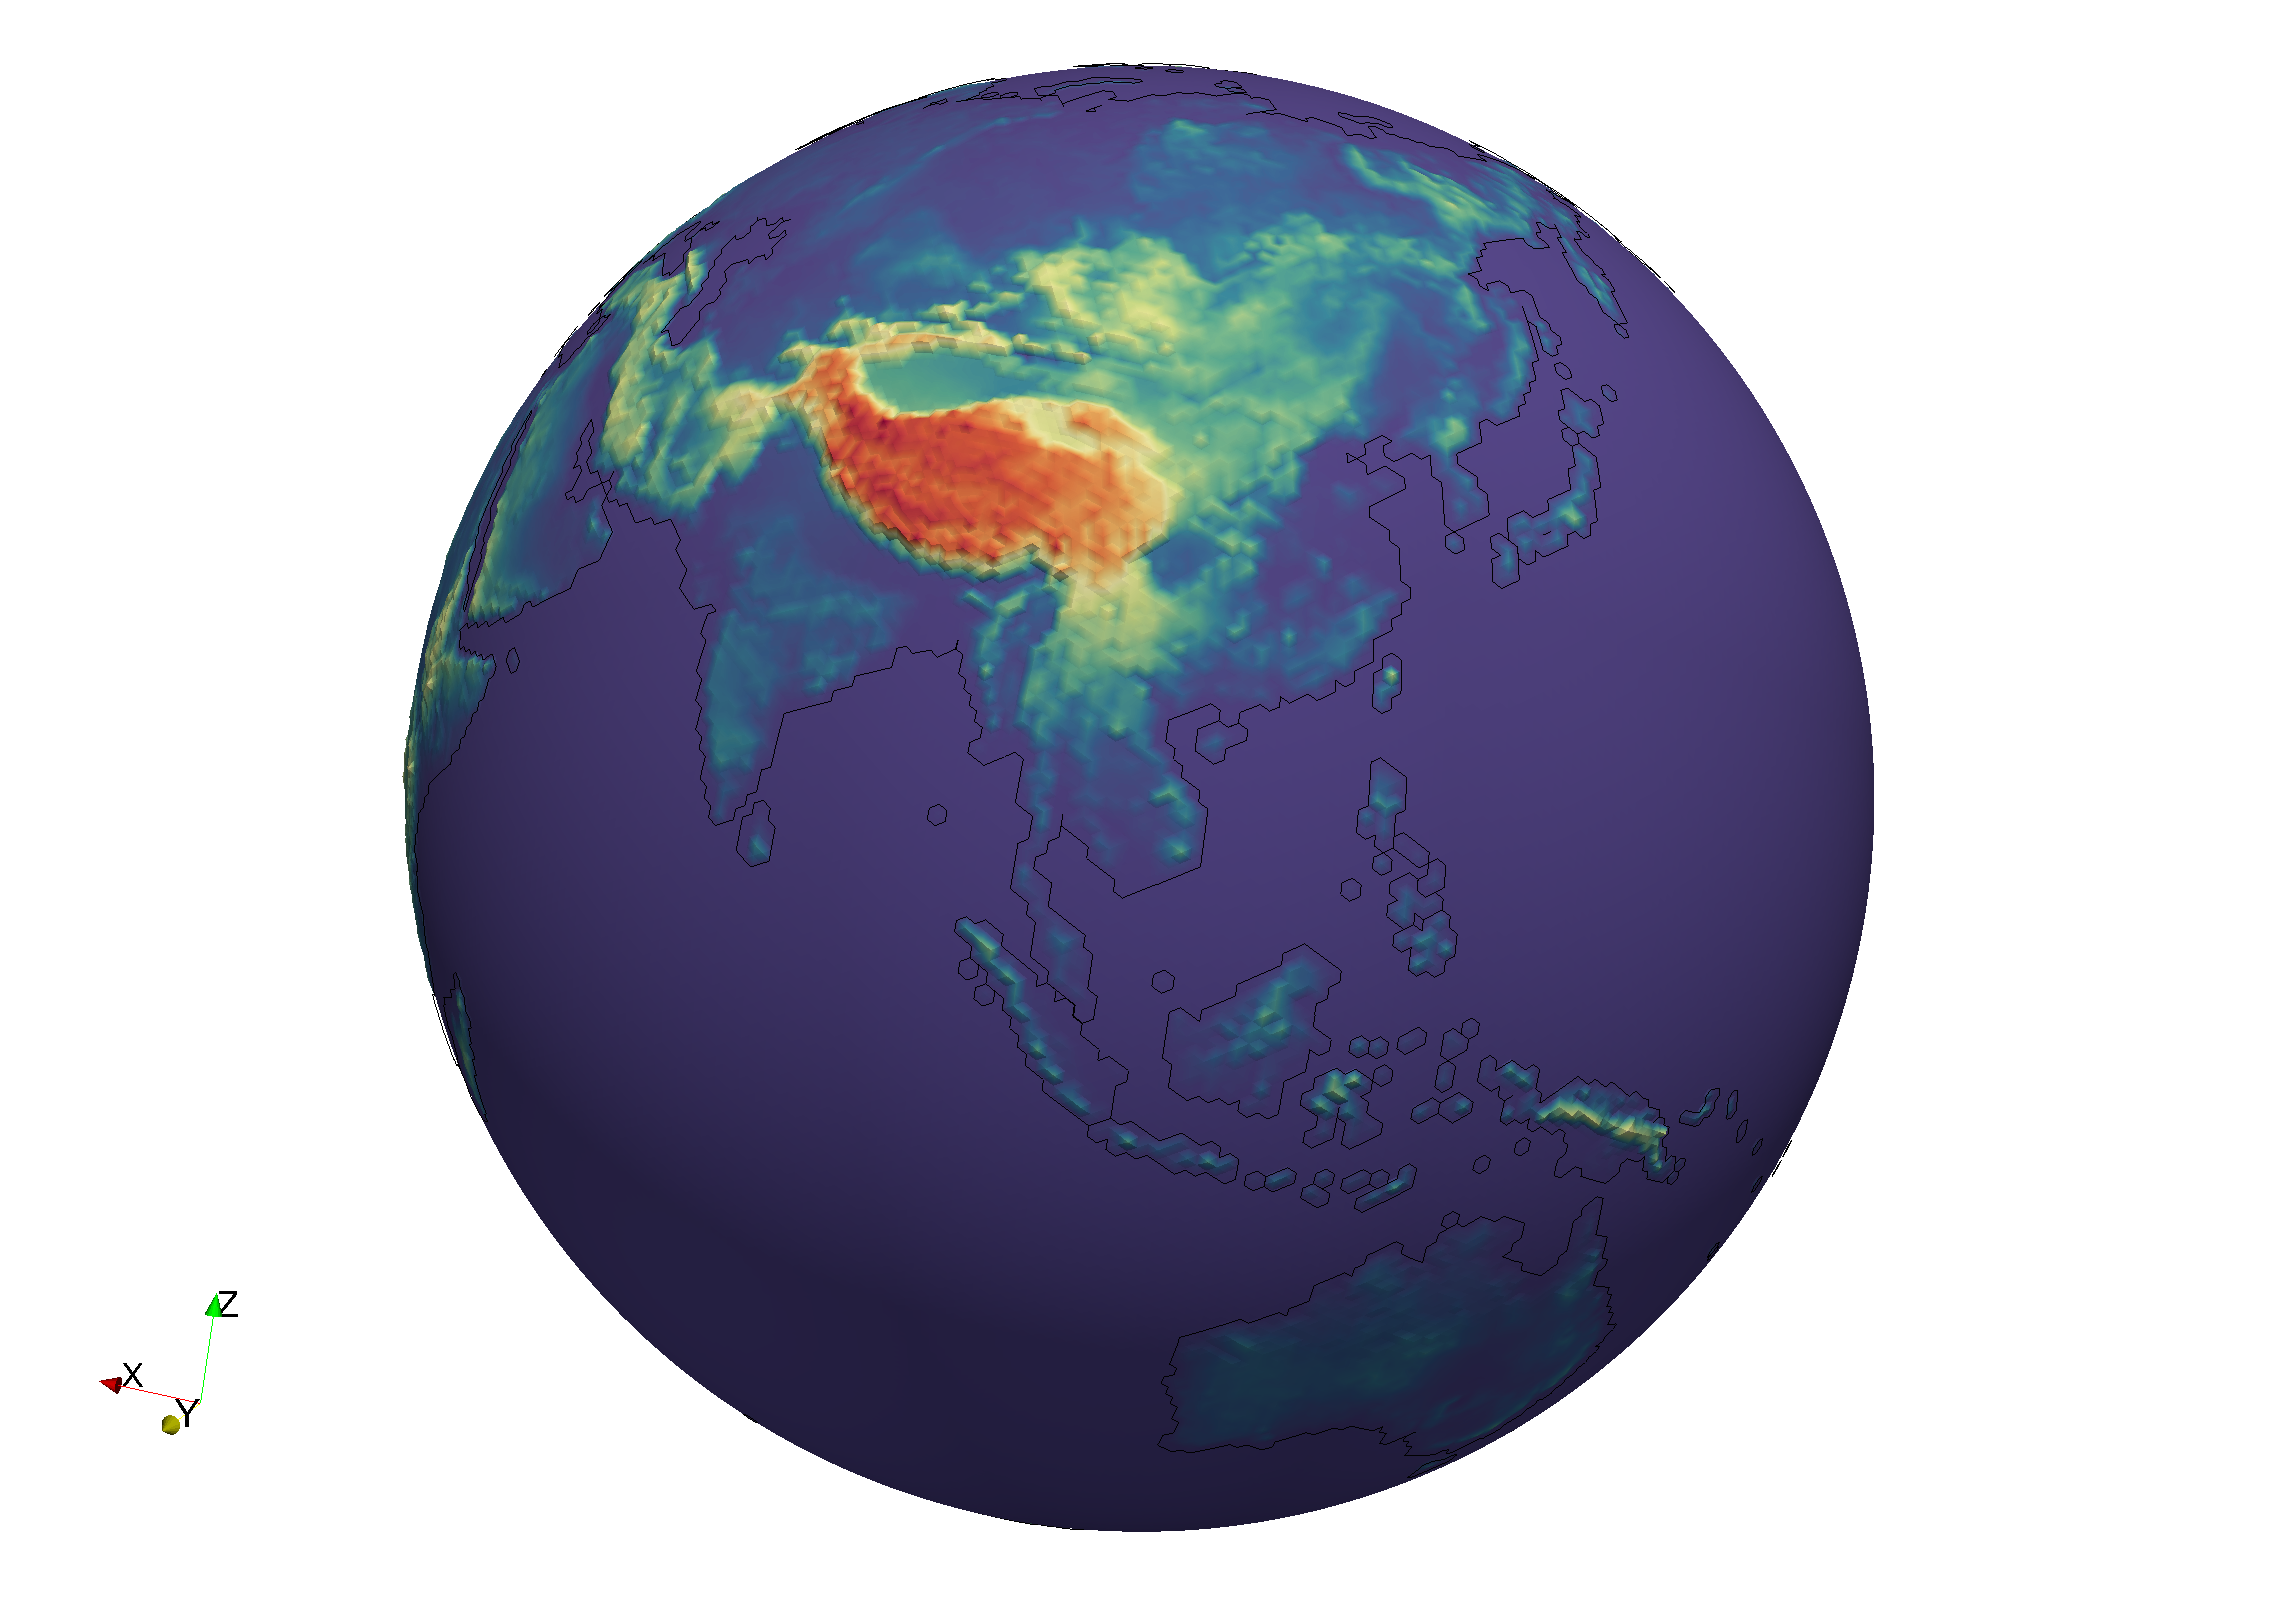
\includegraphics[width=5cm]{python_codes/fieldstone_69/topo/topo3D_2.png}
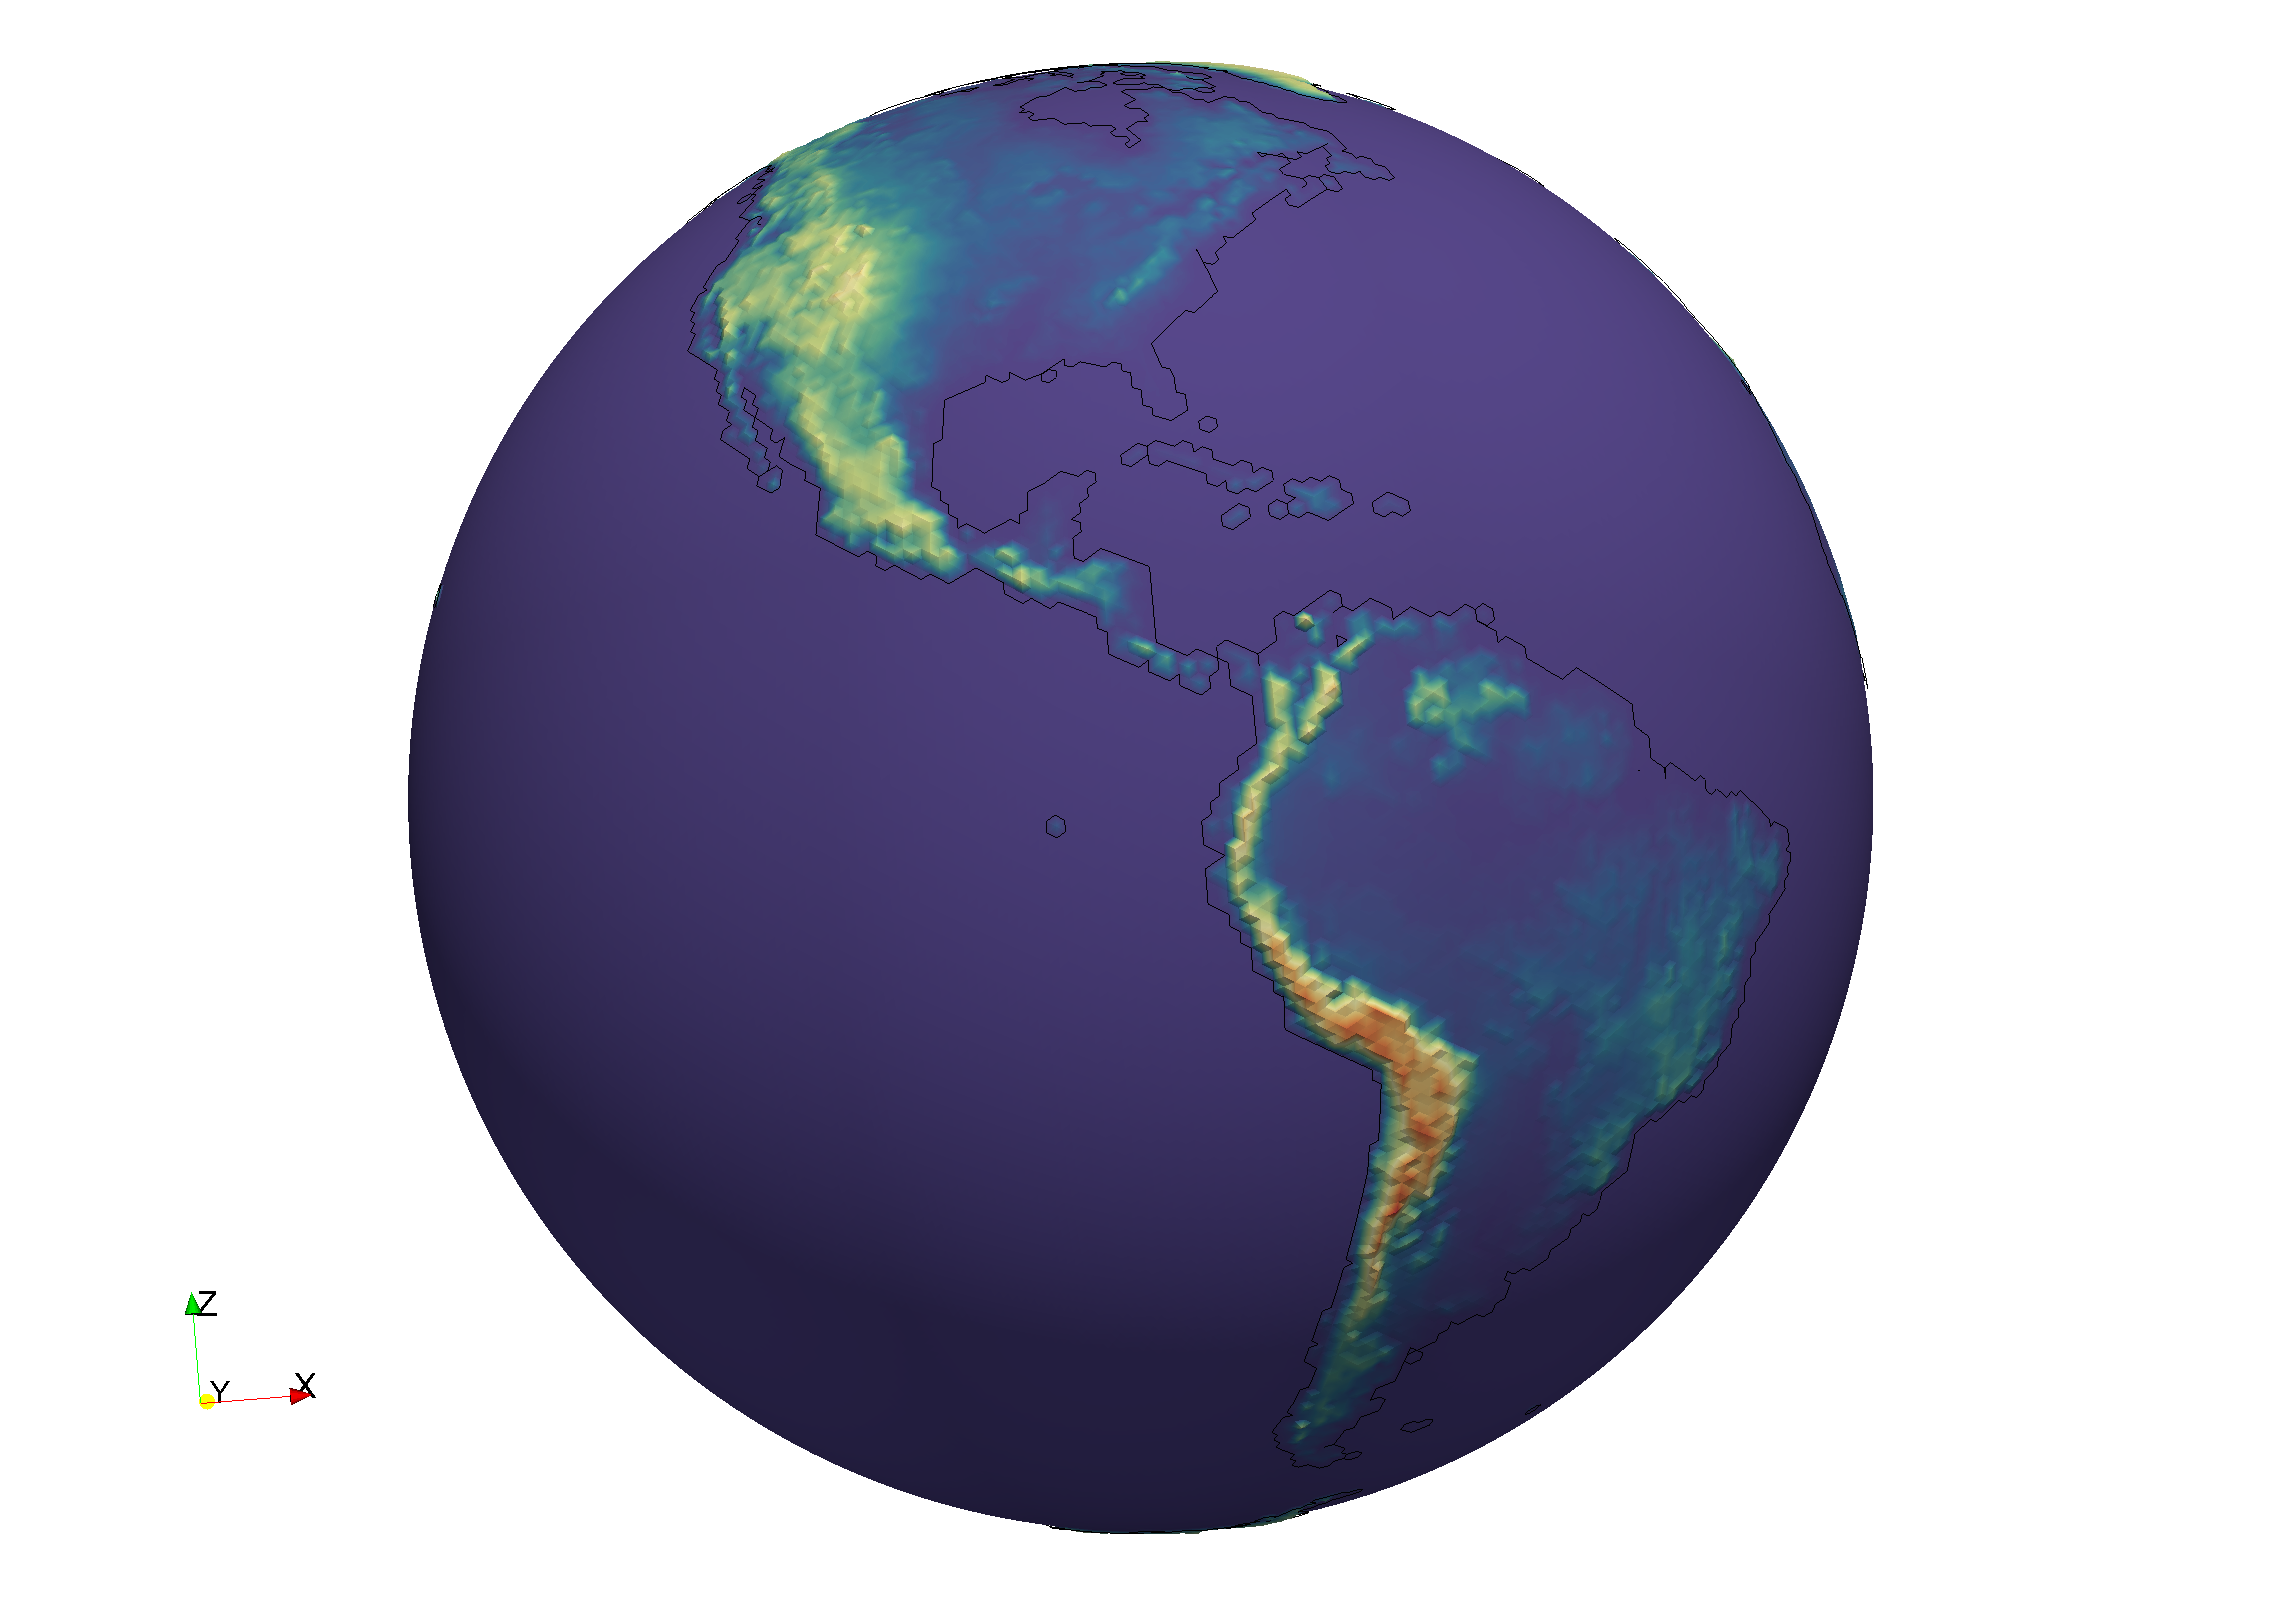
\includegraphics[width=5cm]{python_codes/fieldstone_69/topo/topo3D_3.png}\\
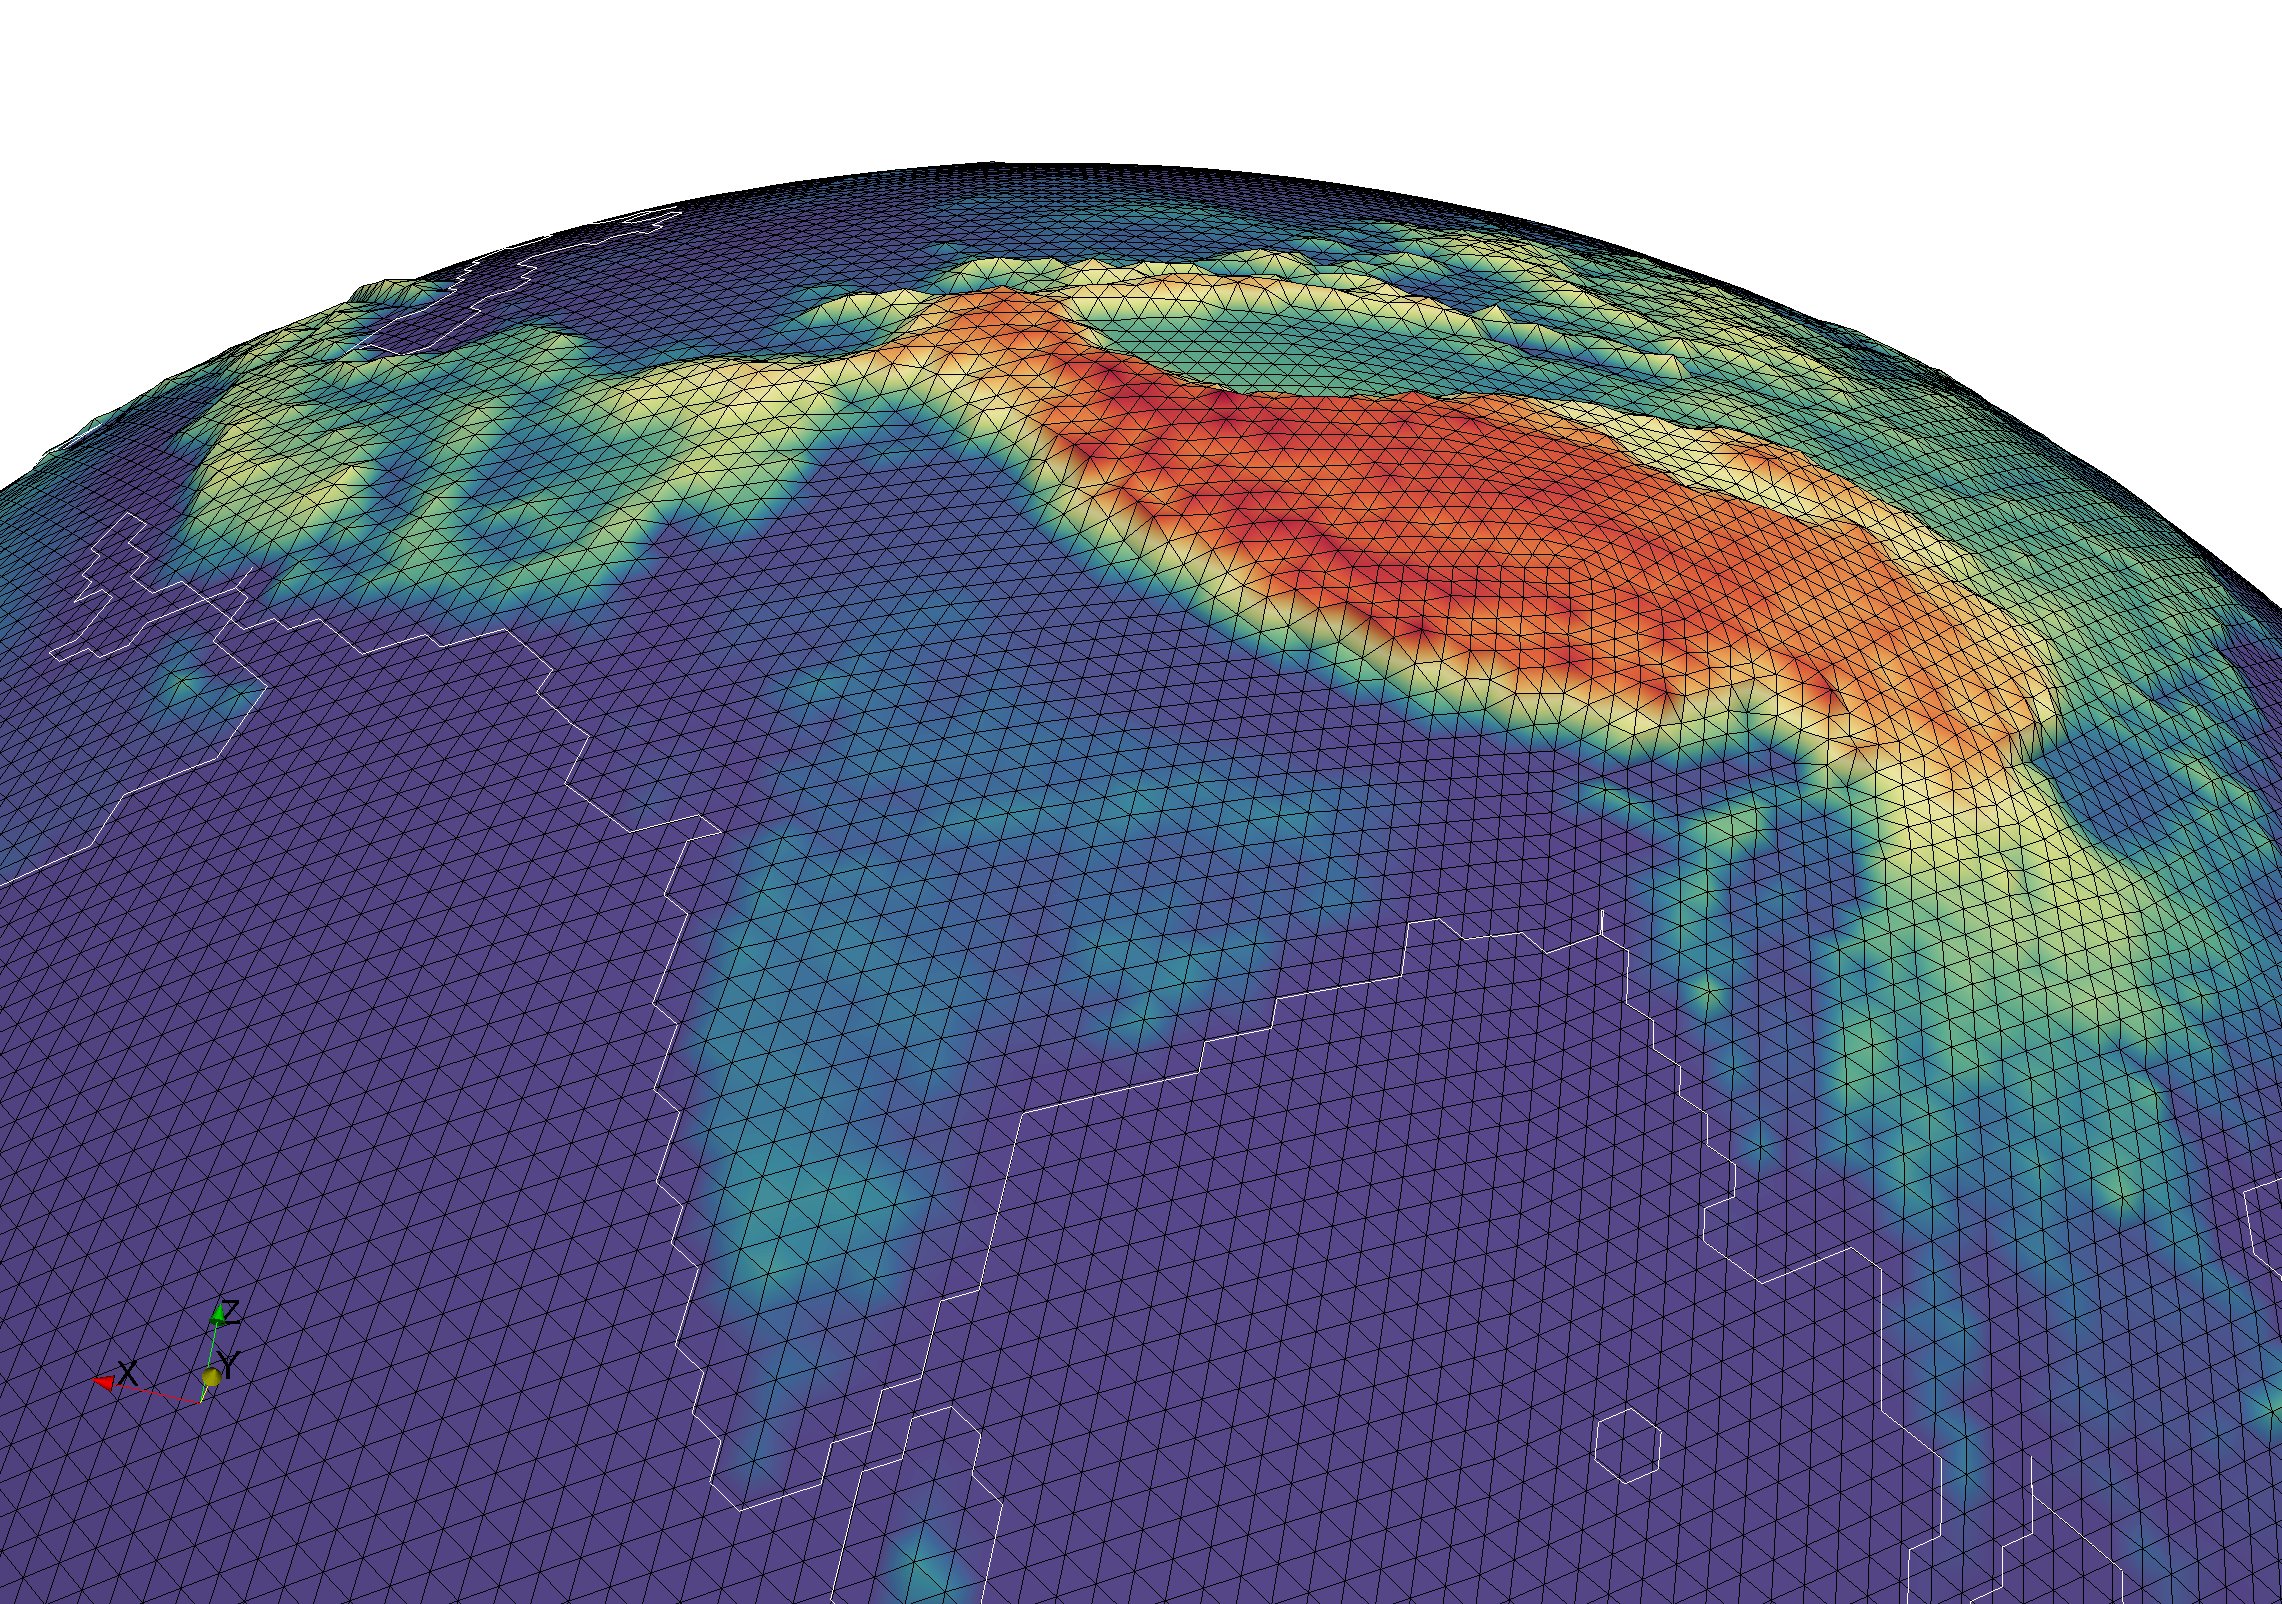
\includegraphics[width=7cm]{python_codes/fieldstone_69/topo/topo3D_4.png}
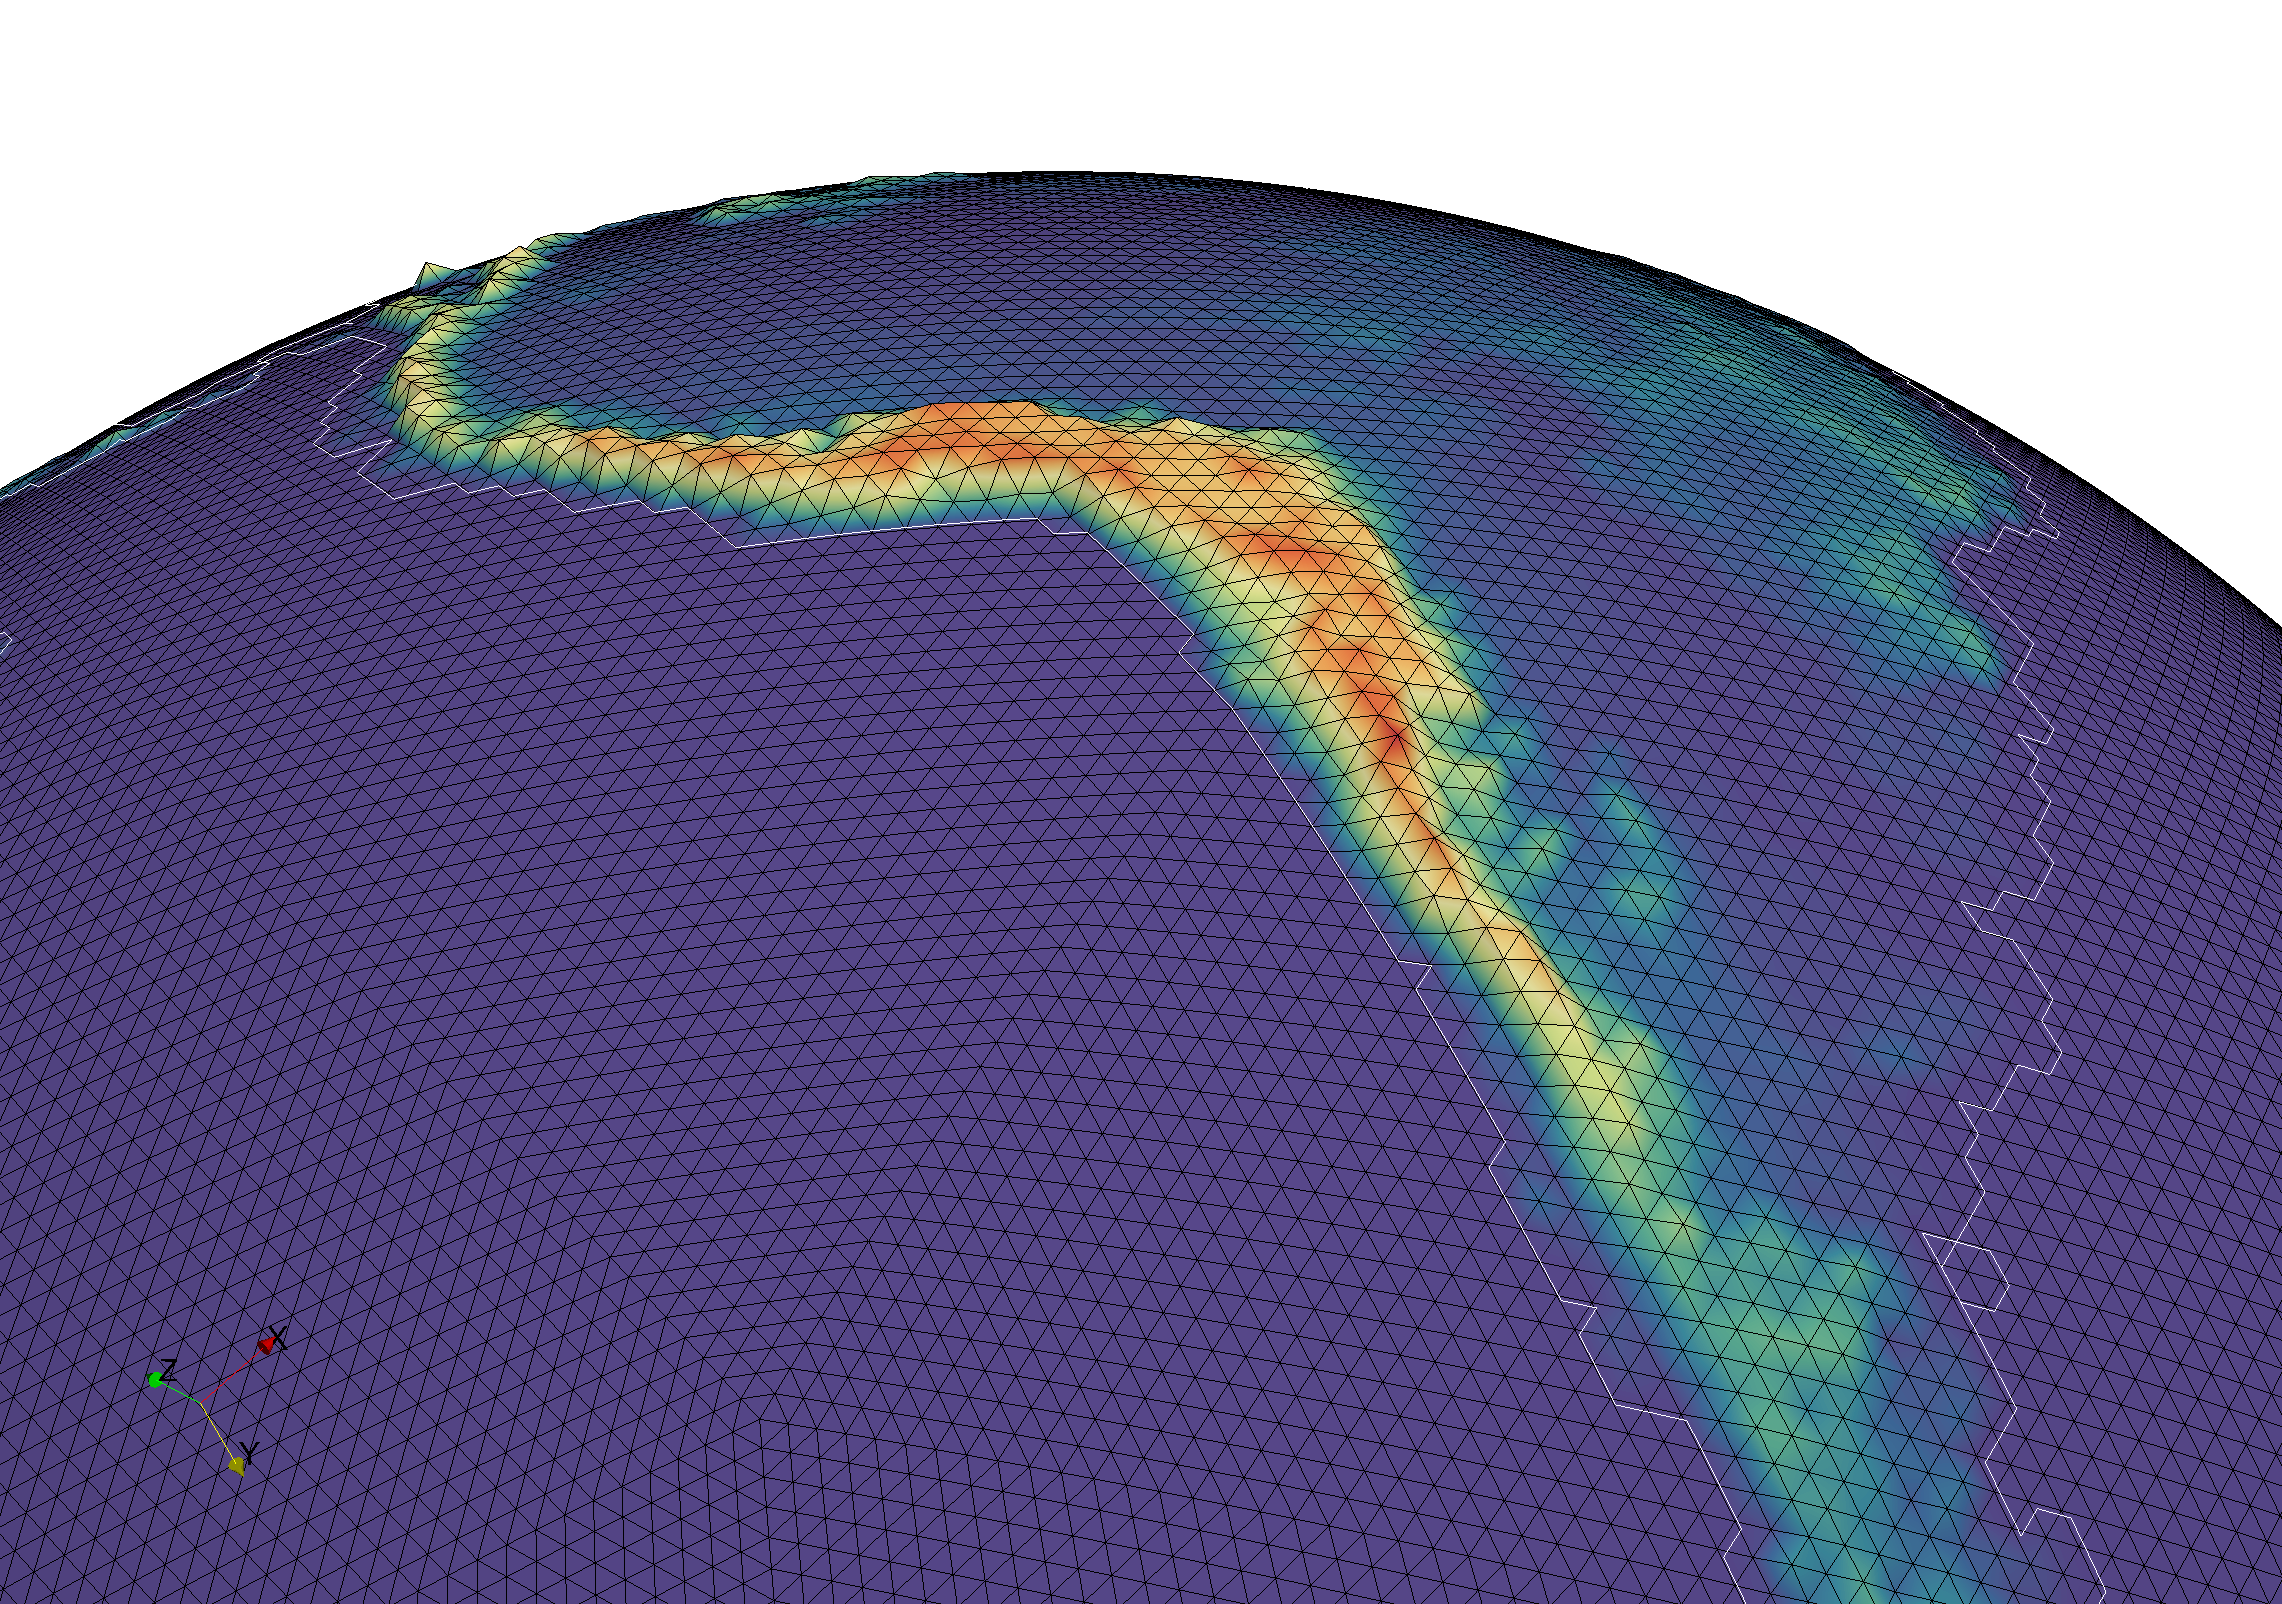
\includegraphics[width=7cm]{python_codes/fieldstone_69/topo/topo3D_5.png}\\
{\captionfont Icosahedral mesh, level=100. Vertical exaggeration=20.}
\end{center}


\begin{center}
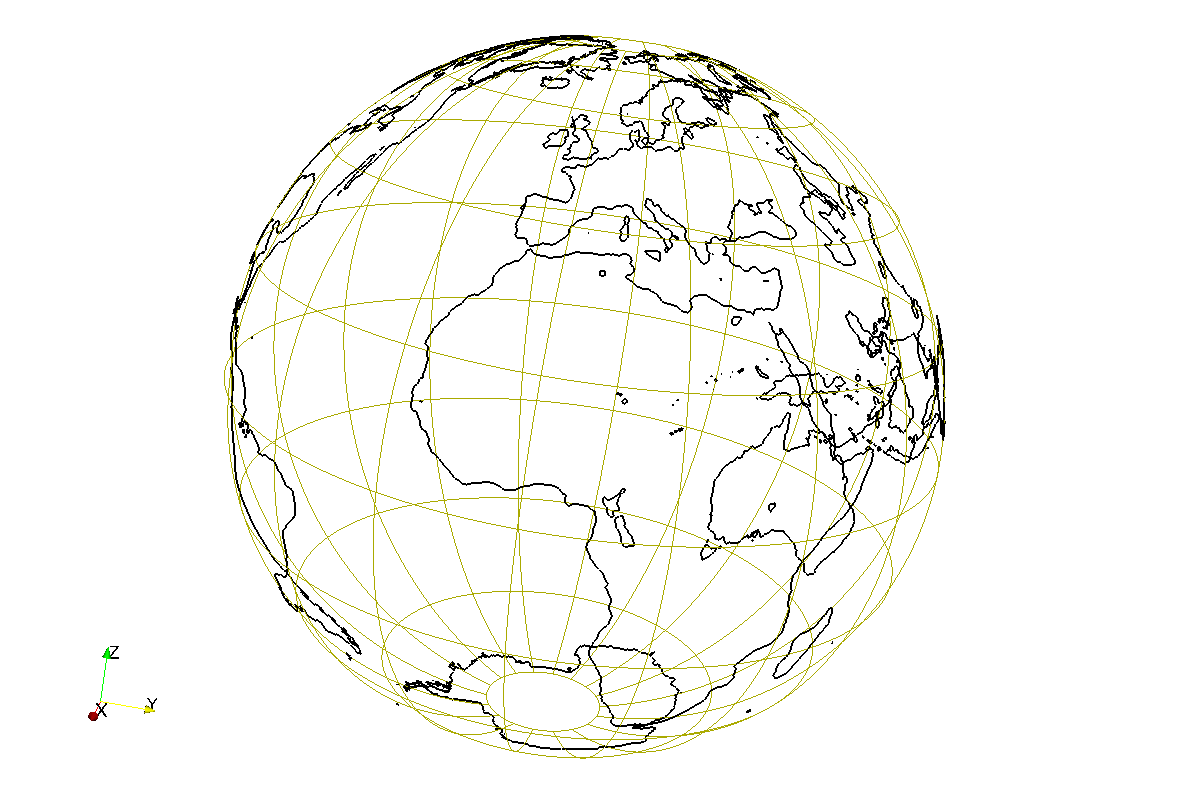
\includegraphics[width=10cm]{python_codes/fieldstone_69/images/coastlines_gridlines}\\
{\captionfont Los Alamos coastlines with grid lines.}
\end{center}

Coastlines, plate boundaries, topography, grid lines available at \url{https://www.earthmodels.org/}.
